%===============================================================================
% LaTeX sjabloon voor de bachelorproef toegepaste informatica aan HOGENT
% Meer info op https://github.com/HoGentTIN/latex-hogent-report
%===============================================================================

\documentclass[english,dit,thesis]{hogentreport}
\usepackage{morewrites}
\usepackage{lipsum}

\graphicspath{{../graphics/}}

\usepackage[chapter,outputdir=../output]{minted}
\usemintedstyle{solarized-light}
\usepackage{float}
\usepackage{capt-of}

\usepackage[automake,acronym,toc]{glossaries}
\makeglossaries
%%=============================================================================
%% Lijst van afkortingen / Glossary of acronyms
%%=============================================================================

\newacronym{lora}{LoRa}{Long Range}
\newacronym{lpwan}{LPWAN}{Low Power Wide Area Network}
\newacronym{css}{CSS}{Chirp Spread Spectrum}
\newacronym{sf}{SF}{Spreading Factor}
\newacronym{ism}{ISM}{Industrial, Scientific and Medical}
\newacronym{rssi}{RSSI}{Received Signal Strength Indicator}
\newacronym{snr}{SNR}{Signal-to-Noise Ratio}
\newacronym{pdr}{PDR}{Packet Delivery Rate}
\newacronym{psk}{PSK}{Pre-Shared Key}
\newacronym{poc}{PoC}{Proof of Concept}
\newacronym{aprs}{APRS}{Automatic Packet Reporting System}
\newacronym{dmr}{DMR}{Digital Mobile Radio}
\newacronym{tdma}{TDMA}{Time-Division Multiple Access}
\newacronym{bipt}{BIPT}{Belgisch Instituut voor Postdiensten en Telecommunicatie}
\newacronym{aes}{AES}{Advanced Encryption Standard}
\newacronym{ctr}{CTR}{Counter (mode)}
\newacronym{los}{LOS}{Line of Sight}
\newacronym{etsi}{ETSI}{European Telecommunications Standards Institute}

\setminted{%
    autogobble,
    frame=lines,
    breaklines,
    linenos,
    tabsize=4,
    fontsize=\small
}

\renewcommand\listoflistingscaption{%
    \IfLanguageName{dutch}{Lijst van codefragmenten}{List of listings}
}
\renewcommand\listingscaption{%
    \IfLanguageName{dutch}{Codefragment}{Listing}
}
\renewcommand*\listoflistings{%
    \cleardoublepage\phantomsection\addcontentsline{toc}{chapter}{\listoflistingscaption}%
    \listof{listing}{\listoflistingscaption}%
}


%%---------- Document metadata -------------------------------------------------
\author{Simon Dierickx}
\supervisor{Mr. S. Van Impe}
\cosupervisor{Mr. M. Aubert}
\title%
    {To what extent does Meshtastic,\\ as a decentralized LoRa-based mesh network, offer a reliable and readily\\ deployable emergency communication solution\\ when primary network infrastructure fails?}
\academicyear{\advance\year by -1 \the\year--\advance\year by 1 \the\year}
\examperiod{2}
\degreesought{\IfLanguageName{dutch}{Professionele bachelor in de toegepaste informatica}{Bachelor of applied computer science}}
\partialthesis{false}

\hyphenation{back-slash}

%% The bibliography (style and settings are  found in hogentthesis.cls)
\addbibresource{bachproef.bib}            %% Bibliography file
\addbibresource{../voorstel/voorstel.bib} %% Bibliography research proposal
\defbibheading{bibempty}{}

%% Prevent empty pages for right-handed chapter starts in twoside mode
\renewcommand{\cleardoublepage}{\clearpage}

\renewcommand{\arraystretch}{1.2}

%% Content starts here.
\begin{document}

%---------- Front matter -------------------------------------------------------

\frontmatter

\hypersetup{pageanchor=false} %% Disable page numbering references
%% Render a Dutch outer title page if the main language is English
\IfLanguageName{english}{%
    %% If necessary, information can be changed here
    \degreesought{Bachelor of applied computer science}%
    \begin{otherlanguage}{dutch}%
       \maketitle%
    \end{otherlanguage}%
}{}

%% Generates title page content
\maketitle
\hypersetup{pageanchor=true}

%%=============================================================================
%% Voorwoord
%%=============================================================================

\chapter*{\IfLanguageName{dutch}{Woord vooraf}{Preface}}%
\label{ch:voorwoord}
This thesis is the last part of my Applied Computer Science education specialising in System and Network Administration at the University of Applied Sciences Ghent (HoGent).
The topic combines multiple of my interests, my initial thesis at Easi couldn't be pursued but I'm happy with the opportunity I had to end up with this topic.

One of the reasons I chose this topic is the opportunity to build my own infrastructure and be able to test it in real life instead of a lab environment.
The way global networks, antennas, etc. work has always fascinated me, and working on this particular thesis allowed me to deepen my knowledge.
On top of this, the current context of geo-political events and the growing risk of natural disasters triggered my curiosity to explore the available possibilities for keeping communication alive in these catastrophic scenarios.

These interests, combined with the opportunity to build some small stuff (waterproofing, soldering, etc.) made this a clear choice for me.

I would like to take this chance to thank my supervisor, Mr.\ S.\ Van Impe, and my co-supervisor, Mr.\ M.\ Aubert of Accenture, for supporting the topic and providing feedback from a security perspective.
I am also grateful to the owners of the hotel/brasserie ``Floreal Le Panoramique'' on Mont-Saint-Aubert for allowing me to install the relay node there.
Without which the measurements of the thesis would have been way more restrained.
Finally, I thank my family and friends for the occasional help I received, serving as a second pair of eyes at the receiving end of a test message or a second pair of hands during the installation process.
%%=============================================================================
%% Samenvatting
%%=============================================================================

% TODO: De "abstract" of samenvatting is een kernachtige (~ 1 blz. voor een
% thesis) synthese van het document.
%
% Een goede abstract biedt een kernachtig antwoord op volgende vragen:
%
% 1. Waarover gaat de bachelorproef?
% 2. Waarom heb je er over geschreven?
% 3. Hoe heb je het onderzoek uitgevoerd?
% 4. Wat waren de resultaten? Wat blijkt uit je onderzoek?
% 5. Wat betekenen je resultaten? Wat is de relevantie voor het werkveld?
%
% Daarom bestaat een abstract uit volgende componenten:
%
% - inleiding + kaderen thema
% - probleemstelling
% - (centrale) onderzoeksvraag
% - onderzoeksdoelstelling
% - methodologie
% - resultaten (beperk tot de belangrijkste, relevant voor de onderzoeksvraag)
% - conclusies, aanbevelingen, beperkingen
%
% LET OP! Een samenvatting is GEEN voorwoord!

%%---------- Nederlandse samenvatting -----------------------------------------

\IfLanguageName{english}{%
\selectlanguage{dutch}
\chapter*{Samenvatting}

Hedendaagse maatschappij is zeer sterk afhankelijk van bestaande netwerkinfrastructuur, ook voor noodcommunicatie.
Wanneer deze infrastructuur uitvalt, hetzij door een storm, stroomonderbreking, grootschalig incident of een bewuste afsluiting (oorlog, etc.), is er nood aan een back-up plan dat onafhaneklijk van deze infrastructuur werkt.

Dit back-up plan moet snel en makkelijk inzetbaar zijn, eveneens betaalbaar op grote schaal en moet zonder vergunning kunnen worden gebruikt.
Er bestaan oplossingen zoals APRS, DMR en andere satelliet alternatieven, maar deze voeldoen niet aan minstens één van deze voorwaarden.

Met deze bachelorproef wordt onderzocht hoe Meshtastic (een gedecentraliseerd mesh-netwerk op basis van LoRa-radiotechnologie) een eventueel alternatief zou kunnen zijn.
Het onderzoek bestaat niet enkel uit een literatuurstudie maar ook uit een werkeleijke real-world opzet tijdens een proof of concept, tijdens deze PoC werden drie nodes opgezet: een vaste basisnode is Ronse, een relay-node in Doornik en een mobiele node.
Gedurende drie testsessies werden zowel het bereik, de signaalsterkte (RSSI), signaalkwaliteit (SNR) en het aantal verloren pakketten (PDR) gemeten.
Dit voor directe verbindingen met de basis node als met de relay node.

Uit deze metingen bleek dat een directe verbinden van 18.5\,km in deze situatie haalbaar is.
Met de huidige setup en beperkingen kon een relay node dit uitbreiden tot ongeveer 30\,km.
Na de relay node in te schakelen werden sommige "dead zones" ook omgeschakeld naar werkende zones.
Een van de belangrijke vondsten, is dat de zichtbaarheid meer impact heeft op het signaal dan de effectieve afstand of de hoogte van de nodes.
De ingebouwde AES-256 encryptie beschermt de inhoud van de berichten, maar het standaardkanaal is publiek en moet dus verwijderd worden.

Binnen een beperkte range, of een grotere ongehinderd oppervlak kan Meshtastic dus een geloofwaardig, goedkoop en onafhankelijk alternatief bieden voor noodcommunicatie.

\selectlanguage{english}
}{}

%%---------- Samenvatting -----------------------------------------------------
% De samenvatting in de hoofdtaal van het document

\chapter*{\IfLanguageName{dutch}{Samenvatting}{Abstract}}

Current society is heavily dpeendent on existing network infrastructure, also for emergency communication.
When this infrastructure fails, due to a storm, power outage, large-scale incident or a deliberate shutdown (wars, etc.), there is a need for a back-up communication system, working independently from the main infra.

This back-up needs to be quick and easy to deploy, as well as affordable on larger scales and should be usable without a license.
Solutions like APRS, DMR and other stellite alternatives exist, but they fail to meet at least one of the mentioned requirements.

With this thesis an investigation of how Meshtastic (a decentralized mesh network based on LoRa radio technology) could be a potential alternative was conducted.
The research doens't only consist of a literature study, but also a real-world deployed proof-of-concept, during which three nodes were deployed: a fioxed base node in Ronse, a relay node in Tournai and a mobile node.
During three distinct test sessions, the range, signal strength (RSSI), signal quality (SNR) and packet loss (PDR) were measured.
These metrics were collected for both direct connections to the base node, as well as connections through the relay node.

From these measurements a direct connection of 18.5\,km with the base node was found achievable in this situation.
Witht he current setup and its limitations, the relay node could extend this range to about 30\,km.
After putting the relay node into the network, some "dead zones" were also found working now.
One of the main findings of the PoC is that line-of-sight matters more than distance or height of the nodes.
The built-in AES-256 encryption protects the content of the messages, even though the default channel stays public, and should be removed on first use during real deployment.

In a limited range, or in larger unobstructed areas, Meshtastic can be a credible, low-cost, independent alternative for emergency communication.

%---------- Inhoud, lijst figuren, ... -----------------------------------------

\tableofcontents

% In a list of figures, the complete caption will be included. To prevent this,
% ALWAYS add a short description in the caption!
%
%  \caption[short description]{elaborate description}
%
% If you do, only the short description will be used in the list of figures

\listoffigures

% If you included tables and/or source code listings, uncomment the appropriate
% lines.
\listoftables

\listoflistings

\printglossary[type=\acronymtype,title={List of Abbreviations}]

% Als je een lijst van afkortingen of termen wil toevoegen, dan hoort die
% hier thuis. Gebruik bijvoorbeeld de ``glossaries'' package.
% https://www.overleaf.com/learn/latex/Glossaries

%---------- Kern ---------------------------------------------------------------

\mainmatter{}

% De eerste hoofdstukken van een bachelorproef zijn meestal een inleiding op
% het onderwerp, literatuurstudie en verantwoording methodologie.
% Aarzel niet om een meer beschrijvende titel aan deze hoofdstukken te geven of
% om bijvoorbeeld de inleiding en/of stand van zaken over meerdere hoofdstukken
% te verspreiden!

%%=============================================================================
%% Inleiding
%%=============================================================================

\chapter{\IfLanguageName{dutch}{Inleiding}{Introduction}}%
\label{ch:inleiding}


Modern society relies heavily, we could even say entirely, on the permanent availabiltiy of our communication netwroks.
Everything has switched to global networks, the Internet, cellular data, phone networks, etc. Everything became embedded in day-to-day life that people use it without even thinking about it, we take it for granted.
Everything means even emergency response depends on said networks to communicate and to coordinate first responders, warn people and keep citizens connected.
This means that this dependcy can becoime critical at the exact moment it is most needed, when networks become unavailable.

When a big storm destroys a cellular tower, or when floods cut power of a specific region (where bases might be running) or other large-scale incidents happen that infrastructure just disappears, and suddenly what we took for granted is no longer available.
This is not just hypotetical; natural disasters, power outages, conflict situations (disrupting traffic, censoring, etc.), these are moments when using the network is necessary, but impossible.

For those exact situations a back-up system should be available. Not only for first responders or civil protection but also for the general public.
A fallback available to the public should be quick and easy to deploy, not require a specialist and be affordable enough.
Several technologies already exists, but they all have their limiations which make them difficult to effectively applu in an emergency.
These limitations can be cost, licences, needed hardware, extra fees, etc.

Thios bachelor thesis will investigate \textbf{Meshtastic}. \textbf{Meshtastic} is an open-source project that allows to build a decentralized, encrypted mesh network. This can be done on low-cost \gls{LoRa} radio hardware.
Meshtastic doesn't require any SIM card, internet connection or lcience. It provides self-healing multi-hop routing which allows us to extend the initial coverage without needing any fixed existing infrastructure.
For these exact reasons, Meshtastic might be a promising candidate for the emergency contexts described above. However real-world tests have been conducted a real emergency reliability and emergency hasn't been evaluated yet. This thesis will address that gap in research by creating a PoC in the region around Ronse, Belgium.
\section{\IfLanguageName{dutch}{Probleemstelling}{Problem Statement}}%

\label{sec:probleemstelling}

Whenever the main infrastructure fails, the responsible people for coordinating instructions, help, etc. are left without any way to do this.
The core problem of this thesis if the absence of an accessible, affordable, reliable and easy to deploy solution that functions independtly of the failed infraastrructure.
Also no evidence is available about how well Meshtastic handles this role in practice.

The primary audience are IT professionals that are responsible for continuity and civil protectiuon communication, such as security teams etc.
As a secondary audience we could also identify volunteer oprganizations, municvipal safety services and network engiuveers who want to investigate low-sot, off the grid coimmunication options.
A last additional audience could just be general public, for who privacy matters and don't want to roam on a controlled network.

\section{\IfLanguageName{dutch}{Onderzoeksvraag}{Research question}}%
\label{sec:onderzoeksvraag}

The central research question of the thesis is: 
\begin{quote}
\emph{To what extent does Meshtastic, as a decentralized \gls{LoRa}-based mesh network, offer a reliable and readily
deployable emergency communication solution when primary network infrastructure fails?}
\end{quote}

From this main question two domains can be identified: the problem and solution domain.

The \textbf{problem domain} is examining the requirements that occur whenever infrastructure fails and how existing solutions address these.
To do this following sub-questions will be answered:
\begin{itemize}
  \item What gaps exist in emergency contexts when the primary infra becomes unavailable?
  \item How do existing alternatives compare to Meshtastic in terms of accessibility, cost, required expertise, etc.?
  \item What environmental factors of the Belgian (Flemish Ardennes and Wallonia) landscape and terrain affect LoRa performance once deployed?
  \item How secure is the Meshtastic encryption in case of traffic interception?
\end{itemize}

The \textbf{solution domain} on the other hand is evaluating the measurements from the real-life deplooyement during the PoC.
This provides us these sub-questions:
\begin{itemize}
  \item What range and reliability does a Meshtastic network have across different topologies (direct long-distance
  vs.\ multi-hop) in a real deployment (East Flanders/Hainaut province: Flemish Ardennes/Pays des Collines regions (Ronse/Oudenaarde/Kluisbergen/Tournai))?
  \item How does the Meshtastic security model hold up against potential attacks?
  \item How does it compare with other alternatives in terms of requirements in emergency situations?
\end{itemize}

\section{\IfLanguageName{dutch}{Onderzoeksdoelstelling}{Research objective}}%
\label{sec:onderzoeksdoelstelling}

There are two goals for this thesis.
First off, using literature, comparing Meshtastic to the most relevant alternatives (being APRS, DMR and other commercial satelitte messengers).
The second one, making use of the \gls{poc}, measuring Meshtastic's effective range, reliability and deployabvility in a real-life mixed terrain.

What the concrete deliverables are:
\begin{itemize}
  \item A requirements list and comparison matrix
  \item A working three or four node Meshtastic deployment (fixed base node, fixed relay node(s) and a mobile node)
  \item A report of field measurements collected during PoC test sessions (range, \gls{rssi}, \gls{snr}, \gls{pdr} and hop count)
  \item A final matrix comparing Meshtastic to the alternatives
\end{itemize}

Success for this thesis can be defined as being able to give a clear, evidence-based answer to the research question, sup^ported by th efield measuremnts the PoC provided.

\section{\IfLanguageName{dutch}{Opzet van deze bachelorproef}{Structure of this bachelor thesis}}%
\label{sec:opzet-bachelorproef}

The structure of this thesis is as follows:

Chapter~\ref{ch:inleiding} introduces the main problem, questions and ideas.

%TODO
\chapter{\IfLanguageName{dutch}{Stand van zaken}{State of the art}}%
\label{ch:stand-van-zaken}

This chapter is an introduction to the current state of the research domain, it examines it in depth.
Establishing what emergency comunication acxtually requires when primary infrastructure fails in the first place (Section~\ref{sec:sota-requirements}). Then reviewing existing relevant off-grid alternatives, APRs in section~\ref{sec:sota-aprs}, DMR in section~\ref{sec:sota-dmr}, and other possible satellite messengers in section~\ref{sec:sota-satellite}.
The rest of the chapter will provide technical background which is necessary to understand the PoC: \gls{lora} (Section~\ref{sec:sota-lora}), Meshtastic architecure (Section~\ref{sec:sota-meshtastic}) and the Meshtastic secuirty model (Section~\ref{sec:sota-security}).
The chapter will close with a comparison evaluated before (Section~\ref{sec:sota-comparison}).

\section{Requirements for emergency communication}%
\label{sec:sota-requirements}

Before anything can be evaluated, let's define emergency communication demands. When the primary infra fails (such as cellular or internet)), the replacement provided should satisfy a list of reqsuirements that is different form our everyday solutions.
The needs identifieds are usually the same, \textcite{ManojBaker2007} state that one of the primary challenges is responding to disasters itself. The tools responders and public use should be affordable, available and usable in daily life.
In a review of communication technologies for difficult terrain they test robustness, rapid deployability, cost and energy eggiciency as well as quality criteria \autocite{ElKhaledMcheick2019}.
The five criteria listed below are the ones used throughout this thesis.

The first and maybe most important, requirement is \textbf{the independence from fixed infrastructure}. If a solution is found but it only works relying on the cnetral tower or on a data centre the same failure as the outage is selected. Which means the solution is unsable.
This is exactly what motivates us to find an autonomous solution \autocite{ManojBaker2007}.

Another requirement is \textbf{quick and easy deployability}. If there is a crisis, there is no time for licences, specialists or training.
The emergency solution shoudl be setupped and ready by "general public" in minutes using the right documentation and instructions.

The thrid requirement is \textbf{affordability at scale}. Only if there are enough participants the emergency solution is useful, which means if buying in to this network is impossible for most "normal" people, then the solution in itself in not usefula t all.
This applies to subscription and per-message fees based solutions as well, especially for larger scale operations.

Range and reliability, are off course one of the main requirements. The solution muist be able to cover a meaningful distance in order for it to be realistically deployable. 
Meaning that in a real-life scenario and terrain, messages should be delivered with an acceptable success rate, with ideally a possiblity to extend it's range if necessary.
Especially in situations where the duration and scope of the emergency is unknown or undetermined.

The last main requirement found is the \textbf{security and privacy} of said solutions. Ins ome specific cases (wars, censorship, etc.) the communication could contain sensitive infromation which shuldn't be intercepted and might be targeted by attacks/snooping.
As discussed in section~\ref{sec:sota-security}, this is desirable, but it isn't always as straightforward as it seems.

These five requirements form the main evaluation cirteria for this thesis. They will be used to compare different alternatives as a solution for the main research question.

\section{APRS (Automatic Packet Reporting System)}%
\label{sec:sota-aprs}

APRS is a known protocol, it's used with amateur radio frequencies, enabling real-time communication of position and telemetric info on said shared frequencies \autocite{UN2023APRS}.
It is however relevant to emergency contexts as it operates independently from the internet. \textcite{UN2023APRS} demonstrates this in a real-world disaster (this happened in Cambodia). Both the response and mobile station operators relied on license amateur radios.

The license is in fact the biggest barrier to rapid dpeloyment, in a conflict scenario those licences could be revoked or the frequencies seized by the authorities. And in case of a natural disaster, there is most likely no time gonna be spent on giving out radio licneces.
It also depends on specialized hardware, which makes it diffuicult to configure and place, especially in crisis conditions. If we compare this to the previously mentioned requirements, APRS is infrastructure independent, but it fails for the eays and quick deploy.

\section{DMR (Digital Mobile Radio)}%
\label{sec:sota-dmr}

DMR, just like APRS, is a protocol base don radio, namely digital mobile radio standard as defines in \textcite{ETSI2023DMR} by the \gls{etsi}.
It is defined in three tiers:
\begin{itemize}
    \item Tier-I: licence-free, low-power, short-range
    \item Tier-II: licensed, \gls{tdma} equipment (voice and IP data), repeater-based communication 
    \item Tier-III: licensed, trunked, \gls{tdma} equipment (voice and IP data), repeater-based communication
\end{itemize}

\textcite{Nyawose2025DMR} confirms the improvements in efficiency, quality and security DMR offers, this compared to analogue radio.

It is however not a suitabel solution for emergency communication.
Tier-I is definitely not suitable because of the severe range limiations. Tier-II and III require licenses, which is one of the main requirements and place it in the same position as APRS.
The dependence on specialized hardware is once again limiting the deplolyment, especially because it's also dpeenden on repeaters, which may be failing due to the same outage as the primary infrastructure.
DMR satisfy range and reliabiltity, but it fails for licensing and deployability.

\section{Satellite messengers}%
\label{sec:sota-satellite}

Commercial satellite based messnegers (e.g. Garmin inReach, Zoleo, Bivy Stick, SPOT, etc.) provide a genuenly off-grid solution, relying on satellite infrastructure instead of terrestrial infrastructure. 
The principal advantage they have over any other solution is the global coverage, which makes the range requirmeent completely irrelevant.

This technology, with all the advatanges it has, isn't something that is easily accessible to everyone. The devices are really expensive and on top of the inital purtchase amount a subscription fee adds up.
Some of these also possess a per-message fee on top of the previously mentioned amounts. This means it's impossible to scale, especially fo rgeneral public associations like volunteer orghanizations or municipal safety services. Especially the recurring cost make it almost imlpossible to dpeloy at scale.
The satellite messengers satifsfy the independency and range requirmeents, but horrendously fail on affordability at scale.

\section{LoRa}%
\label{sec:sota-lora}

Before diving into the whole Meshtastic architecture, it's important to understand the technology it is built on, \gls{lora}.
\gls{lora} is a physical-layer protocol that modulates radio signals in the \emph{"sub-GHz"} ISM band, these are free to use and unlicensed frequencies. To modulate they use \gls{css}, which is developed and sold by Semtech \autocite{Raza2017LPWAN}.
How it works is, instead of sending on a fixed narrowband,\gls{lora} spreads the input signal over a wider channel using chirps. This reuslts in noise-like properties on the signal, which makes it more resistant to interferences, and make distant nodes able to decode the signal even if the signal is heavily polluted by noise.

To achieve this, the \gls{sf} parameter is configured. It ranges from 6 to 12 and controls the balance between range and data rate.
A higher \gls{sf} means longer chirps which means higher range, but lower data rate. The \gls{sf} combined with the bandwith and coding rate determines the sensitivity and the througput \autocite{Raza2017LPWAN}.
The hardware used in this thesis (Heltec V4 with Semtech SX1262 tranceiver) has a maximum sensitivity of $-148$ dBm, which is achieved with a \gls{sf} of 12.

\gls{lora} comes with some limitations as well, in Europe it only allows operation on the 868 MHz band. it is also subject of duty-cycle and power limitations. These are defined by \gls{etsi}, and in Belgium by \gls{bipt}. 
These limitations directed us in the right direction for the used config in the \gls{poc}, this can be found in chapter~\ref{ch:methodologie}.

\gls{lora} in itself isn't how the nodes form a entwork, this is just a modulation protocol. The most known layer built on top of \gls{lora} is \gls{lpwan}, more specifically the LoRaWAN protocol.
It organizes end-devices in a star-topology network around fixed gateways. This dependency on gateways introduces the same exact main indrastructure dependence problem as the other solutions. Here is where Meshtastic shows a different approach.

The usage of \gls{lora} for off-grid emergency communciation has been explored, for example in \textcite{Hochst2020LoRa}, they evaluate \gls{lora}-based communciation for crisis situations. This showed a ranges of 4.6 to 6.5\,km, with a base node placed on a high building (dpeending on the used antenna and frequency).
This provides a useful comparison to the measuremnts in chapter~\ref{ch:poc}.

\section{Meshtastic}%
\label{sec:sota-meshtastic}

Now \gls{lora} has been explained, the base of Meshtastic is clear. Meshtastic itself is an open-source firmware that turns simple microcontrolelrs (mostly ESP32) into nodes of a decentralized mesh network \autocite{MeshtasticDocs}.
It has attracted academic attentiuon oiver the last few years as an off-grid emergency alternative: \textcite{SepulvedaMeshtastic2026} analyzes the resilience of Meshtastic networks and it's modem presets in logn)range propagation scneraios, coriming that each node can act as a router and a client. Unlike LoRaWAN, it doesn't depend on gateways, each node can both create forward and receive traffic.
The network is also self-healing, this means that the route automatically adjusts whenever a node appears or disappears. This is really useful in emrgency cases, where a node can suddenly be unavailable or be added.
Each node is independent, it require no SIM card, no internet connection and no licence.

Different roles can be attributed to the nodes, a \texttt{CLENT} node is an endpoint operated by a user; a \texttt{ROUTER} nodes is optimized to only relay traffic and a \texttt{CLIENT\_BASE} node combines both, it allows the node to forward traffic while also being able to connect to a user as an end-device.
Message go from one node to another, with a maximum hop limit you can set up in the app.

Meshtastic puts nodes into different channels, each channel is named, encrypted and defined by a \gls{psk} \autocite{MeshtasticChannels}.
A device wanting to participate in said channel, must have the smae channel name and \gls{psk} configured. Eight different channels can be configured on a single node simultaneously, one primary and seven seocndary channels, each with its own key \autocite{MeshtasticChannels}.

\begin{figure}
  \centering
  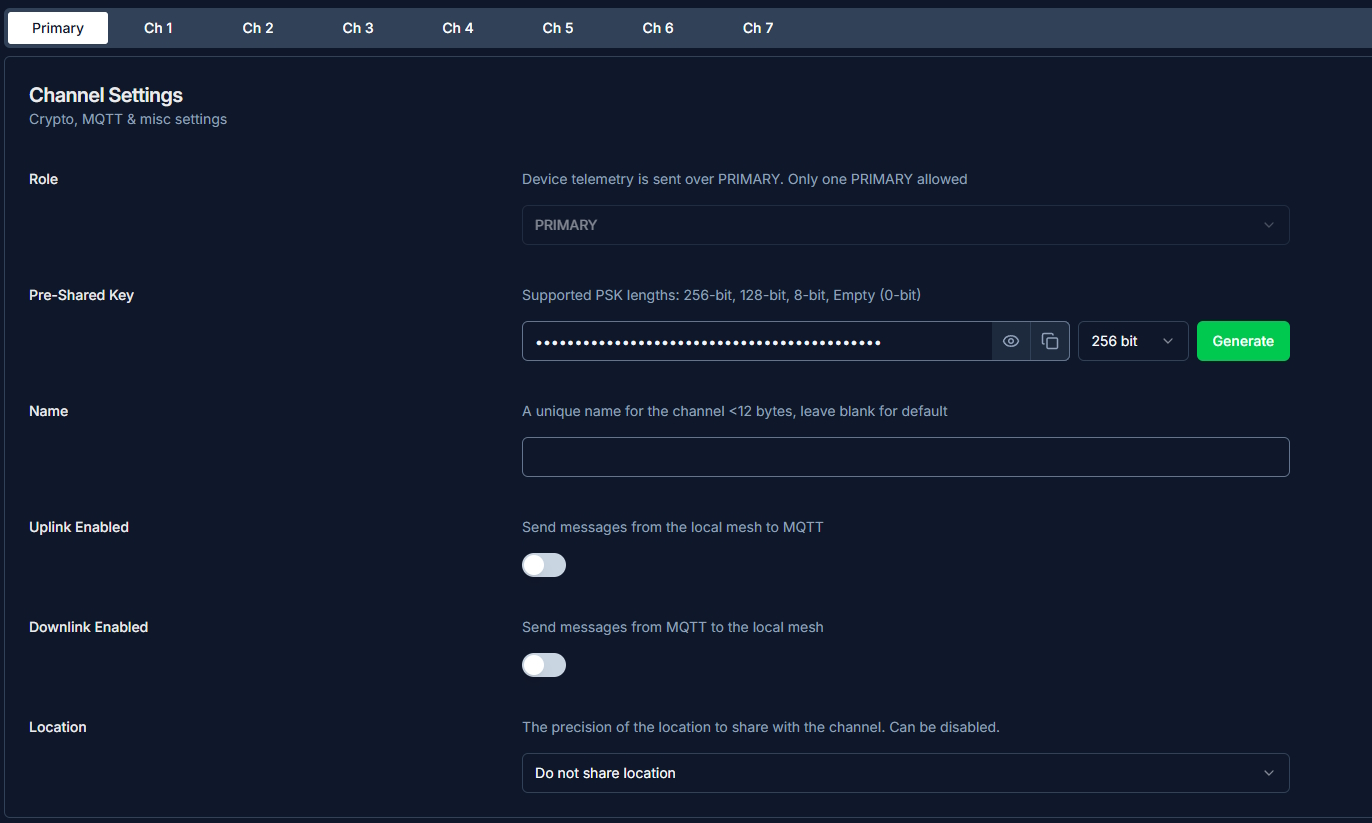
\includegraphics[width=0.8\textwidth]{meshtastic-channels.jpg}
  \caption[Meshtastic channels config.]{\label{fig:meshtastic-channel}Primary and seocndary channels with their respective options.}
\end{figure}

The above mentioned properties are the ones that make Meshtastic a potential candidate for our problem. It's inexpensibve, licence-free, quick to deploy, all of this falls into the deployability and affordabilityu requirements that were defined earlier. The questions left to answer to check if Meshtastic is in fact a suitabel candidate are: range, reliability and security in emergency cases.

\section{Meshtastic security model}%
\label{sec:sota-security}

One of the subquestions was the secuirty of Meshtastic in case of traffic interception. 

\section{Comparative overview}%
\label{sec:sota-comparison}



%%=============================================================================
%% Methodologie
%%=============================================================================

\chapter{\IfLanguageName{dutch}{Methodologie}{Methodology}}%
\label{ch:methodologie}

In this chapter the plan of execution will be explained.
The exact execution was split up in five distinct phases.
For each phase the objective, deliverables and research methods are described.
The execution and results of the \gls{poc} are only described in Chapter~\ref{ch:poc}.

\section{Phase 1: Literature study}%
\label{sec:method-literature}

The first of the five phases is a literature study. This means through research in available documentation answers are formulated on the problem-domain sub questions.
Establishing requirements for emergency communication, reviewing existing alternatives (\gls{aprs}, \gls{dmr} and satellite messengers) as well as the known technical aspects of \gls{lora} and Meshtastic.
Those digital sources are evaluated using the CRAAP test (Currency, Relevance, Accuracy, Authority and Purpose).
The deliverables are a requirements list (Section~\ref{sec:sota-requirements}) and the comparison explained in Chapter~\ref{ch:stand-van-zaken}.
Together they focus on the cost, licensing, range, reliability, ease of config and deployability.

\section{Phase 2: Design of the proof of concept}%
\label{sec:method-design}

In this second phase the goal was designing a \gls{poc}. Starting by selecting the appropriate hardware, number of necessary nodes, and their roles. As required (by \gls{bipt}) the config was limited to the EU\,868\,MHz band.

As clean \gls{los} was expected to be an important factor a three-node topology was designed, consisting of two elevated fixed nodes (base and relay).
The third node was then a mobile node so testing could easily be done and compared to one another.
The reasoning, difficulties and setup is documented in Chapter~\ref{ch:poc}.

\section{Phase 3: Execution and measurement}%
\label{sec:method-measurement}

Third phase is the effective execution of the \gls{poc}: the field tests.
Two different topologies were tested:
\begin{enumerate}
  \item \textbf{Topology 1 (direct link)}: during this test only two nodes were used, this was to test the direct connection between the base
  node and the mobile node. This was used to establish the maximal single-hop range of the network.
  \item \textbf{Topology 2 (relay link)}: for this test the three-node topology was used. After finding the best spot for the relay
  using the first topology, this one was to test the coverage of the entire network from base to relay to mobile node.
  This way the extension of the range using a multi-hop path was determined.
\end{enumerate}

Two built-in instruments from the Meshtastic firmware helped during the drive.

The \emph{Range Test} module was configured on the mobile node. This module communicates a test packet every 60 seconds from the moment the mobile node is booted.
These packets are numbered and contain a series of metrics: timestamp, GPS coordinates (when a phone is connected), \gls{rssi} and \gls{snr} values. These packets
are sent to the base node where a CSV file can be extracted. That way you can immediately tell the sequences missing, and as a result the timestamps/locations of no connection.

On top of the Range Test module the \emph{traceroute} function was also used, this wasn't to determine the dead zones while driving like the range test, this is used on the stop locations to test the full path to the base node.
The metrics this gave were: the full path traveled (hops between mobile and base) and the quality of each single hop (\gls{rssi} and \gls{snr} values).

Both these tests combined gave a clear view of coverage (working zones, dead zones) and the quality of the connections.
All those measurements were taken across multiple testing days, different locations, times of day and weather conditions where possible (even though this July/August months in belgium were extremely dry so no real weather difference could be measured).
This was done so that environmental, weather and topological factors were taken into account, and not just based on a single working snapshot.
Each fixed node was powered by a battery and a solar panel, this way running it autonomously could also be investigated.

\section{Phase 4: Security analysis}%
\label{sec:method-security}

For the fourth phase, the encryption sub-question, the main analysis is based on the official Meshtastic documentation.
As described in Section~\ref{sec:sota-security}, the firmware's security model is analysed as well.
No attempt has been made to try and break the encryption itself, both because as seen in the documentation, \gls{aes} is not the weak point and mostly because intercepting and/or decrypting third-party traffic is illegal.
That said, some tests can be done on the field, having an additional node, not part of the network (encrypted with a different key) and see if it gets the traffic to forward it, and try to read the message (which shouldn't be possible because of the encryption).

\section{Phase 5: Comparative analysis}%
\label{sec:method-comparison}

In the fifth and final phase all the collected results are compared with the initial literature findings.
Using the evaluation criteria established during the first phase a scoring matrix will be built.
Based on literature and on the \gls{poc} Meshtastic, \gls{aprs}, \gls{dmr} and satellite messengers are compared. This can be found in Chapter~\ref{ch:conclusie}.
%%=============================================================================
%% Proof of Concept
%%=============================================================================

\chapter{\IfLanguageName{dutch}{Proof of concept}{Proof of concept}}%
\label{ch:poc}

This chapter presents and analyzes the proof of concept.
First is deciding which hardware is selected and the reasoning behind these choices (Section~\ref{sec:poc-hardware}), followed by the
hardware assembly and construction together with the configuration of the nodes and the difficulties encountered during setup (Section~\ref{sec:poc-config}).
The next part is presenting and analyzing the results of three different field-test sessions: direct-link baseline (Section~\ref{sec:poc-session1}), relay survey (Section~\ref{sec:poc-session2}) and full deployment (Section~\ref{sec:poc-session3}).
At the end of this chapter we can also observe other nodes, not known to us participating in the mesh network (Section~\ref{sec:poc-mesh}), the security demonstration (Section~\ref{sec:poc-security}) and the evaluations of autonomous solar operation (Section~\ref{sec:poc-solar}).

\section{Hardware selection}%
\label{sec:poc-hardware}

The main constraint while choosing hardware was cost (this is one of the requirements for emergencies).
The hardware should be able to support EU\,868\,MHz band as this is legally obliged, it should also allow an external antenna for improved range and permit power via battery and solar for autonomous usage.

The final hardware choice was to use the \textbf{Heltec WiFi LoRa 32 V4}. This is a board using an Espressif ESP32-S3 microcontroller and the Semtech SX1262 \gls{lora} transceiver.
Four units were acquired, one base node, one mobile node, one relay and the last one was a spare/second relay node if necessary.
The V4 was chosen over the V3 (cheaper model) because it provides solar-charging input, higher maximum transmit power and the possibility to add a battery.
These features are important in this use case. 
The SX1262 transceiver provides a better sensitivity compared to the SX1276 (used on older models), this is important for long-range usage.

Another important piece of hardware are the antennas. The provided antenna with the board is a small PCB antenna which is unusable in long-range scenarios and if the board is placed in an enclosure.
Having to place the nodes outside this would also mean the antenna is unusable. That's why for the two fixed nodes (base and relay) a 5\,dBi external antenna was chosen. This antenna is omnidirectional which allows us to have a good coverage, despite the orientation.
The main V4 boards were then mounted inside the enclosure and the external antenna was connected using a u.FL-to-SMA cable.
The mobile node was equipped with a 868\,MHz antenna with a magnetic base so that it could be mounted on the car roof.

For realistic emergency situations both the fixed nodes were not plugged in a regular electrical socket. That's why for both the fixed nodes a small 2,000\,mAh/3.7\,V LiPo battery was used as a buffer.
The main power source was a 6\,W 5\,V/1\,A solar panel, the size of this panel (27.1 x 17.5 x 0.26\,cm) allows it to be easily mounted and directed to the sun.
This way the nodes use the solar panel to be powered on and charge the battery during the day, at night or at cloudy weather the battery takes over.
On the base node the solar panel was soldered to a JST\,1.25\,mm connector so the USB-C plug could be used for data transfer.
The mobile node was powered using USB-C from the car.

This setup was then mounted in an IP66 junction box for the fixed nodes.
The junction box protects the hardware against dust and heavy rain and the cable glands allows the antenna and cables to get in and out of the box while being sealed.

Table~\ref{tab:poc-cost} summarizes the cost of the whole operation, as cost is one of the main criteria in these emergency scenarios.
This is a relevant result in itself for the scope of this thesis. The complete setup (four nodes, including a spare node, cables, antennas, batteries, solar panels and enclosures) was acquired for \euro{}180.95 in total.
This was on the chosen sites and at the moment of building the setup in Belgium, prices may vary according to time and location. 

The bought components were not necessarily the cheapest available at the moment on the market, but due to the time constraints this project fell in, some products had to be chosen from more expensive EU-based resellers instead of non-EU resellers, which may be a lot cheaper, in order to achieve it in time.
But even given this, the total cost of the setup compared to the cost of a commercial solution (e.g. a single Garmin inreach device) costs more than the full setup before even paying any subscription or fee.
The figures below represent a realistic upper bound on the cost, this should not be taken as a cost-optimized setup. According to estimations, a total of \euro{}100/150 could be done, according to the amount of nodes needed, etc.

\begin{table}[H]
  \centering
  \small
  \begin{tabular}{lrrr}
    \toprule
    \textbf{Component} & \textbf{Unit price} & \textbf{Qty} & \textbf{Subtotal} \\
    \midrule
    Heltec WiFi LoRa 32 V4 (868\,MHz)          & \euro{}22.00 & 4 & \euro{}88.00 \\
    6\,W USB solar panel (5\,V/1\,A)            & \euro{}19.99 & 2 & \euro{}39.98 \\
    LiPo battery 2,000\,mAh (JST 1.25\,mm)       & \euro{}9.64  & 2 & \euro{}19.28 \\
    Vecys 3\,dBi magnetic-base car antenna      & \euro{}7.87  & 1 & \euro{}7.87  \\
    5\,dBi omnidirectional antenna (2-pack)     & \euro{}6.76  & 1 & \euro{}6.76  \\
    Kopp IP66 enclosure                         & \euro{}5.36  & 2 & \euro{}10.72 \\
    Goobay USB-C to USB-A cable (3\,m)          & \euro{}5.50  & 1 & \euro{}5.50  \\
    DIGITUS USB-A extension cable (3\,m)        & \euro{}1.59  & 1 & \euro{}1.59  \\
    SMA-female to u.FL-female cable (20\,cm)    & \euro{}1.25  & 1 & \euro{}1.25  \\
    \midrule
    \multicolumn{3}{l}{\textbf{Total (four-node kit)}} & \textbf{\euro{}180.95} \\
    \bottomrule
  \end{tabular}
  \caption[Material cost of the \gls{poc} network.]{\label{tab:poc-cost}Material cost of the hardware. Prices are the prices paid at time of purchase. The kit contains four nodes (three effective, one spare) 3 antennas, 2 batteries, 2 solar panels, 2 enclosures and additional cables. Small consumables such as cable glands, silicone and mounting hardware are excluded.}
\end{table}

\section{Physical build and installation}%
\label{sec:poc-build}

The fixed nodes were assembled inside an IP66 junction box. The V4 board was placed with dual-sided tape inside the box, together with the LiPo battery (JST 1.25mm connector).
The 5\,dBi antenna was mounted on the outside of the box using a u.FL-to-SMA cable. The board possesses a second JST 1.25mm connector for solar energy.
The solar panel we used had a USB-A output, we soldered a cut USB-A cable to the JST 1.25mm cable.
For the base node the solar panel was mounted on top of the junction box, for the relay node it was separated to put in an optimal position inside the tower.

The base node was then installed on a house on one of the outskirts of Ronse (50.72316, 3.63217), at an altitude of 90\,m.
The complete setup can be seen in figure~\ref{fig:poc-build-ronse} down below.
The relay node was installed inside the viewing tower of Floreal Le Panoramique on the Mont-Saint-Aubert (50.65457,
3.39975) with an altitude of 140\,m. Permission was obtained from the owners. The installation as seen in figure~\ref{fig:poc-build-relay} shows the solar panel is set up to be facing southwards.
The junction box and antenna are oriented towards the base node.

\begin{figure}[H]
  \centering
  \includegraphics[width=0.8\textwidth]{poc-build-ronse.jpg}
  \caption[Assembled base node.]{\label{fig:poc-build-ronse}The base node inside the junction box and the roof installation. The V4 board, LiPo battery, antenna and solar panel can be identified.}
\end{figure}

The final installation of the relay node looked like this:
\begin{figure}[H]
  \centering
  \includegraphics[width=0.8\textwidth]{poc-build-relay.jpg}
  \caption[Relay installation.]{\label{fig:poc-build-relay}The relay node installation inside the viewing tower of Floreal Le Panoramique.}
\end{figure}

\begin{figure}[H]
  \centering
  \includegraphics[width=0.8\textwidth]{poc-panoramique.jpg}
  \caption[Relay installation + viewing area.]{\label{fig:poc-panoramique}The red marker indicates the position of the base node.}
\end{figure}

No real setup was done for the mobile node. This was powered via the car's USB-C socket, connected to the antenna, magnetically attached to the car's roof.
A phone was connected through Bluetooth to the mobile node, allowing it to broadcast its real-time GPS location.

\section{Configuration and setup difficulties}%
\label{sec:poc-config}

Using the \href{https://flasher.meshtastic.org/}{Meshtastic firmware flasher} the last stable version of Meshtastic (2.7.\allowbreak26.\allowbreak54e0d8d) was flashed on all four nodes.
The board needed the installation of the CH343 driver to be able to flash and configure the board. The Heltec device should also be put into bootloader mode by holding the PRG button while plugging it in.

The nodes can then be configured on three different ways: the web-based configuration interface, the Python command-line interface or the mobile application.

The applied configuration was quite similar and simple on all three nodes.

On all three nodes the radio profile was set on the EU\_868 region, LONG\_FAST modem preset (which is 250\,kHz bandwidth, \gls{sf} 11, coding rate 4/5), a hop limit of 3, a transmit power of 27\,dBm (as allowed in the EU\_868 band),
boosted receiver gain enabled and the FEM/LNA mode disabled (the V4 has no external low-noise amplifier).
However the three nodes received three different roles: base node in Ronse as \texttt{CLIENT\_BASE} (sending, receiving and forwarding messages), relay node as \texttt{ROUTER} (forwarding messages) and mobile node as \texttt{CLIENT} (receiving and sending messages). 
The Meshtastic Range Test module was enabled and configured so that the mobile node was sending a test packet every 60 seconds to the base node. The base node then kept this in a CSV log file for later analysis.
These sequences contained a sequence number, time of reception, \gls{rssi}, \gls{snr} and the exact position of the node (this device doesn't have a GPS module, but it uses the phone's shared GPS position).

For all three nodes current configuration has been set up and saved to the devices:
\begin{table}[H]
  \centering
  \small
  \begin{tabular}{lccc}
    \toprule
    \textbf{Setting} & \textbf{Base-Node (Ronse)} & \textbf{Relay-Node (Tournai)} & \textbf{Mobile Node} \\
    \midrule
    Name                  & Ronse-Base & Relay-Node & Mobile-Node \\
    Role                  & \texttt{CLIENT\_BASE} & \texttt{ROUTER} & \texttt{CLIENT} \\
    Device type           & Heltec WiFi LoRa 32 V4 & Heltec WiFi LoRa 32 V4 & Heltec WiFi LoRa 32 V4 \\
    Firmware version      & 2.7.26.54e0d8d & 2.7.26.54e0d8d & 2.7.26.54e0d8d \\
    Region                & EU\_868 & EU\_868 & EU\_868 \\
    Modem preset          & LONG\_FAST & LONG\_FAST & LONG\_FAST \\
    Bandwidth             & 250\,kHz & 250\,kHz & 250\,kHz \\
    Spreading factor      & 11 & 11 & 11 \\
    Coding rate           & 4/5 & 4/5 & 4/5 \\
    Hop limit             & 3 & 3 & 3 \\
    Transmit power        & 27\,dBm & 27\,dBm & 27\,dBm \\
    Boosted RX gain       & Enabled & Enabled & Enabled \\
    FEM/LNA mode          & Disabled & Disabled & Disabled \\
    Rebroadcast mode      & ALL & ALL & ALL \\
    Power saving          & Off & On & Off \\
    Fixed position        & Yes & Yes & No (phone GPS) \\
    Range Test            & Receiver (CSV) & Receiver & Sender (60\,s) \\
    \bottomrule
  \end{tabular}
  \caption[Meshtastic node configuration.]{\label{tab:poc-config}The exact configuration applied to all three nodes.}
\end{table}

The nodes were properly configured, but this wasn't without any difficulties.
These are also findings of this thesis to take into account (deployability requirement):
\begin{itemize}
    \item The web-based configurator was unreliable for bulk configuring the device. Settings appeared as saved but frequently weren't really saved after the reboot. The Python CLI and mobile application were both more reliable, so that's what was used.
    \item Reflashing the firmware doesn't hard reset the device. A partial or corrupted config survives a reflash and must be manually cleared.
    \item When using the CLI the order and timing of the executed commands should be carefully considered. A reboot might be triggered and some commands get ignored.
    \item Polarity of the LiPo battery connector needs to be checked before installing, apparently this isn't standardized.
\end{itemize}

As mentioned above, the nodes were not always easy to set up using the Web Client, that's why some of the settings were done through the app to stay persistent.
The app, however, is really user-friendly but not as complete as the Web Client could be. That's why the CLI was used to perform some of the more ``advanced'' settings.
As shown below, each of the nodes had such a config file, which was a regular .bat file, pushing the configuration settings on a specified COM-port at the top of the file.

\begin{minted}{batch}
  @echo off
  REM ================================================================
  REM  MESHTASTIC - NODE: RONSE-BASE
  REM ================================================================

  SET COM_PORT=COM4
  SET MESH=python -m meshtastic --port %COM_PORT%

  REM -- Test connection first --
  echo [TEST] Checking connection...
  %MESH% --info > nul 2>&1
  IF ERRORLEVEL 1 (
      echo ERROR: Cannot connect on %COM_PORT%
      echo Check Device Manager for correct COM port number.
      pause
      exit /b 1
  )
  echo OK - Connected.
  echo.

  REM ================================================================
  REM  1. IDENTITY
  REM ================================================================
  echo [1/9] Setting identity...
  %MESH% --set-owner "Ronse-Base"
  timeout /t 3 /nobreak > nul
  %MESH% --set-owner-short "RONS"
  timeout /t 3 /nobreak > nul

  REM ================================================================
  REM  2. LORA RADIO
  REM ================================================================
  echo [2/9] Configuring LoRa radio...
  %MESH% --set lora.region EU_868
  timeout /t 3 /nobreak > nul
  %MESH% --set lora.modem_preset LONG_FAST
  timeout /t 3 /nobreak > nul
  %MESH% --set lora.hop_limit 3
  timeout /t 3 /nobreak > nul
  %MESH% --set lora.tx_enabled true
  timeout /t 3 /nobreak > nul
  %MESH% --set lora.tx_power 0
  timeout /t 3 /nobreak > nul
  %MESH% --set lora.sx126x_rx_boosted_gain true
  timeout /t 3 /nobreak > nul
  %MESH% --set lora.ignore_mqtt true
  timeout /t 3 /nobreak > nul
  %MESH% --set lora.ok_to_mqtt false
  timeout /t 3 /nobreak > nul
  %MESH% --set lora.override_duty_cycle false
  timeout /t 5 /nobreak > nul

  REM ================================================================
  REM  3. FIXED POSITION (Ronse)
  REM     !! Update coordinates to exact installation spot !!
  REM     Right-click on Google Maps -> "What's here?" for exact coords
  REM ================================================================
  echo [3/9] Setting fixed position (Ronse)...
  %MESH% --setlat 50.72306 --setlon 3.63234 --setalt 88
  timeout /t 5 /nobreak > nul
  %MESH% --set position.gps_mode NOT_PRESENT
  timeout /t 3 /nobreak > nul
  %MESH% --set position.broadcast_secs 3600
  timeout /t 3 /nobreak > nul
  %MESH% --set position.smart_enabled false
  timeout /t 5 /nobreak > nul

  REM ================================================================
  REM  4. POWER (mains powered, no saving needed)
  REM ================================================================
  echo [4/9] Power settings...
  %MESH% --set power.is_power_saving false
  timeout /t 3 /nobreak > nul
  %MESH% --set power.wait_bluetooth_secs 0
  timeout /t 5 /nobreak > nul

  REM ================================================================
  REM  5. BLUETOOTH
  REM ================================================================
  echo [5/9] Bluetooth...
  %MESH% --set bluetooth.enabled true
  timeout /t 3 /nobreak > nul
  %MESH% --set bluetooth.mode NO_PIN
  timeout /t 5 /nobreak > nul

  REM ================================================================
  REM  6. DISPLAY
  REM ================================================================
  echo [6/9] Display...
  %MESH% --set display.screen_on_secs 60
  timeout /t 3 /nobreak > nul
  %MESH% --set display.units METRIC
  timeout /t 3 /nobreak > nul
  %MESH% --set display.twentyfourhr_clock true
  timeout /t 3 /nobreak > nul
  %MESH% --set display.heading_bold true
  timeout /t 3 /nobreak > nul
  %MESH% --set display.wake_on_tap_or_motion true
  timeout /t 3 /nobreak > nul
  %MESH% --set display.compass_north_top true
  timeout /t 3 /nobreak > nul
  %MESH% --set display.carousel_delay_sec 5
  timeout /t 5 /nobreak > nul

  REM ================================================================
  REM  7. MODULES
  REM ================================================================
  echo [7/9] Module config...

  REM Telemetry - logs battery voltage over time
  %MESH% --set telemetry.device_update_interval 1800
  timeout /t 3 /nobreak > nul

  REM Neighbor info - logs mesh topology
  %MESH% --set neighbor_info.enabled true
  timeout /t 3 /nobreak > nul
  %MESH% --set neighbor_info.update_interval 3600
  timeout /t 3 /nobreak > nul

  REM Serial debug output
  %MESH% --set serial.enabled true
  timeout /t 3 /nobreak > nul
  %MESH% --set serial.baud 115200
  timeout /t 3 /nobreak > nul

  REM Range test - RECEIVER MODE, saves CSV (thesis measurement data!)
  %MESH% --set range_test.enabled true
  timeout /t 3 /nobreak > nul
  %MESH% --set range_test.sender 0
  timeout /t 3 /nobreak > nul
  %MESH% --set range_test.save true
  timeout /t 5 /nobreak > nul

  %MESH% --set telemetry.device_telemetry_enabled true
  timeout /t 5 /nobreak > nul
  %MESH% --set telemetry.device_update_interval 900
  timeout /t 5 /nobreak > nul

  REM MQTT disabled
  %MESH% --set mqtt.enabled false
  timeout /t 3 /nobreak > nul

  REM ================================================================
  REM  8. DEVICE CONFIG (may cause reboot)
  REM ================================================================
  echo [8/9] Device config (node may reboot after this)...
  %MESH% --set device.rebroadcast_mode ALL
  timeout /t 3 /nobreak > nul
  %MESH% --set device.node_info_broadcast_secs 3600
  timeout /t 3 /nobreak > nul
  %MESH% --set device.tzdef "CET-1CEST,M3.5.0,M10.5.0/3"
  timeout /t 5 /nobreak > nul

  REM Role is set LAST because it always triggers a reboot
  %MESH% --set device.role CLIENT_BASE
  echo Waiting 35 seconds for node to reboot...
  timeout /t 35 /nobreak > nul

  REM ================================================================
  REM  9. VERIFY
  REM ================================================================
  echo [9/9] Verifying configuration...
  %MESH% --info

  echo.
  echo ================================================================
  echo  RONSE-BASE configuration complete.
  echo  Check output above - verify:
  echo    - Owner: Ronse-Base / RONS
  echo    - Role: CLIENT_BASE
  echo    - Region: EU_868
  echo    - Modem preset: LONG_FAST
  echo ================================================================
  echo.
  pause
\end{minted}
\captionof{listing}[Config file]{\label{lst:poc-config-file}Example of a config file from one of the nodes.}


The Python CLI saved lots of time configuring, but also verifying existing config using the following command:

\begin{minted}{batch}
  python -m meshtastic --port {PORT} --info
\end{minted}
\captionof{listing}[Config verification]{Command to verify the nodes configuration.}


\section{Session 1: Direct-link baseline}%
\label{sec:poc-session1}

The first test session consisted of discovering the usage of Meshtastic and \gls{lora} technology, as well as testing a direct link between the Ronse base node and the mobile node.
The first goal was to establish a baseline for a long single-hop connection, without any relay nodes. The secondary goal of this test was also to discover dead zones in the area.
The mobile node was driven from the base to the Mont-Saint-Aubert transmitting a test packet every 60 sec, the base node then logged the received packets so we can check when the node was in a so called ``dead zone''.

Three different phases could be distinguished in the perceived data. The first phase were the first three kilometres from the base node, on similar altitude without any direct line-of-sight.
The \gls{pdr} was 78.6\,\% and the \gls{rssi} degraded from $-51$\,dBm to $-119$\,dBm as the distance increased.
After these initial three kilometres a first complete dead zone was found, lower altitude, no line-of-sight with the home node, these factors made communication impossible, 0\,\% \gls{pdr}.
Eventually the mobile node reached the Mont-Saint-Aubert. This is an elevated part of Tournai with some spots having a clear uninterrupted line-of-sight to the base node.
While ascending the Mont-Saint-Aubert the total \gls{pdr} of the climb was 68.8\,\% and the \gls{rssi} stabilized around $-107$\,dBm with an \gls{snr} of approximately $+1$\,dB.
The maximum distance at which communication was established that day was 18.5\,km.

The key takeaway from this first testing session was that what the distance isn't the real challenge in our scenario. The terrain obstruction and absence of line-of-sight is the main limiting factor for long-range communication with these types of devices.
The dead zone was at 8--15\,km while we had a link at 18.5\,km.
The measured \gls{rssi} $-107$\,dBm also sits within the SX1262 sensitivity of approximately $-132$\,dBm at the LONG\_FAST setting.
This means that there was a $25$\,dBm margin. The \gls{snr} distribution and stability of this link are shown in figures~\ref{fig:poc-snr-hist} and~\ref{fig:poc-snr-stab}.

\begin{figure}[H]
  \centering
  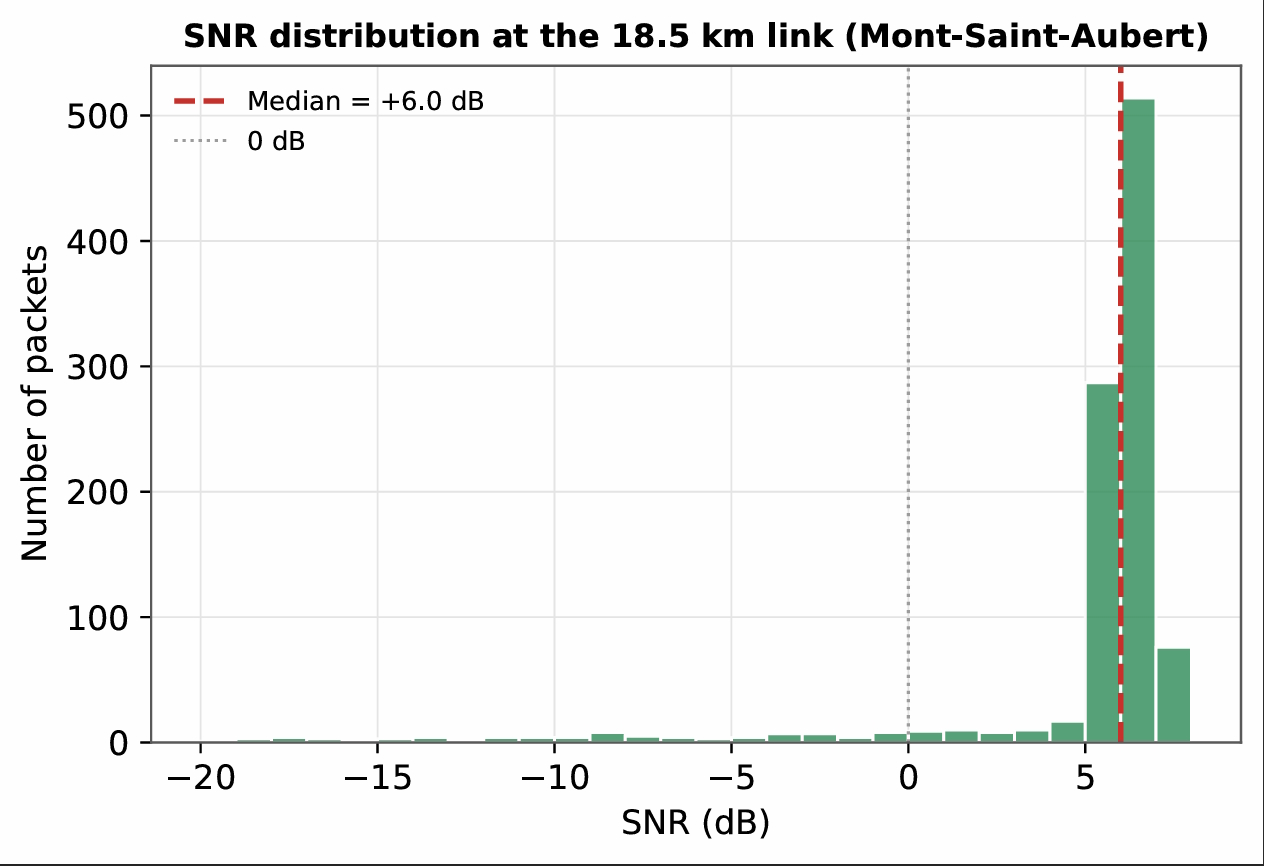
\includegraphics[width=0.85\textwidth]{plot-snr-histogram.pdf}
  \caption[SNR distribution at 18.5\,km.]{\label{fig:poc-snr-hist}\gls{snr} distribution of the 1\,015 packets received during 18.5\,km test at Mont-Saint-Aubert. 91.7\,\% of packets had a positive \gls{snr}, with a median of $+6$\,dB, confirming the maximum-range link was of consistently high quality.}
\end{figure}

\begin{figure}[H]
  \centering
  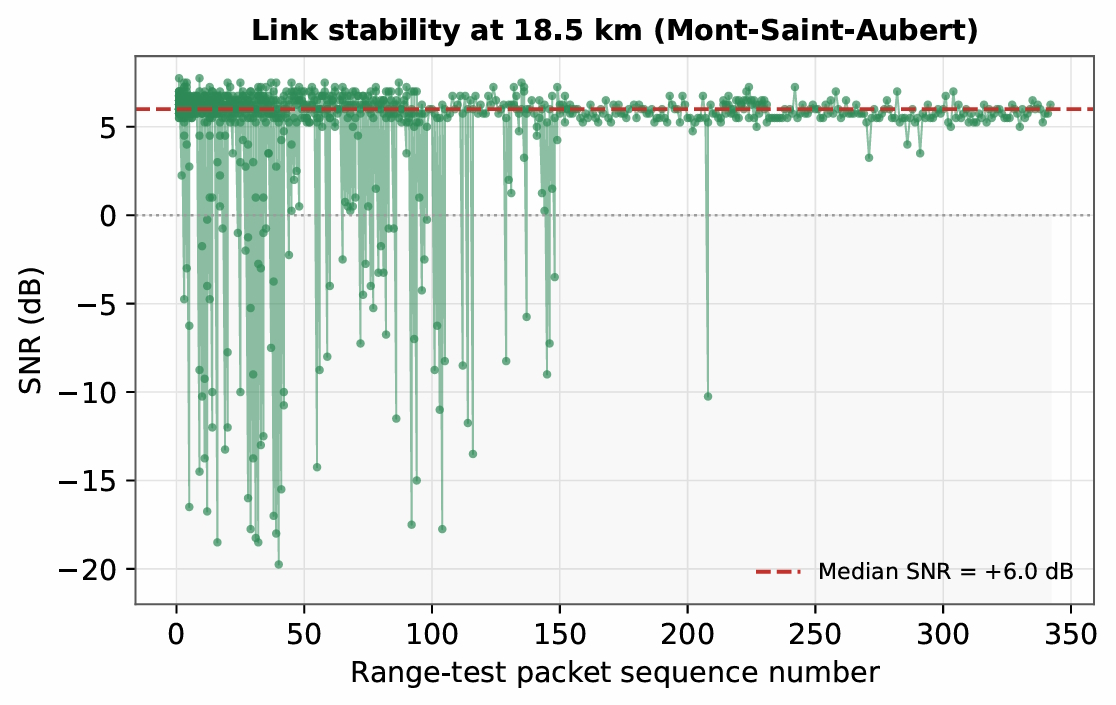
\includegraphics[width=0.85\textwidth]{plot-snr-stability.pdf}
  \caption[Link stability at 18.5\,km.]{\label{fig:poc-snr-stab}\gls{snr} across the range-test packets during the 18.5\,km test. After some initial variation, the link stabilised around $+6$\,dB and delivered 341 of 342 packets (99.7\,\% \gls{pdr}), showing the maximum-range link was sustainable.}
\end{figure}

\section{Session 2: Relay-candidate survey}%
\label{sec:poc-session2}

The second test session focused on other directions from the base node, with the same goal, finding a good location for the relay.
The first session focused mainly on a southern/south-western direction. This second session focused on a northern/north-western direction.
East wasn't checked because the eastern area starting from the node is densely planted with trees and elevation goes even higher at some points.

The locations checked were around the Hotond, Kwaremont, Trieu and Kanarieberg. Most locations are all elevated and have a somewhat clear line-of-sight with the base node.
At each location the \gls{rssi}, \gls{snr} and \gls{pdr} on the direct link to the base node were recorded, together with the altitude and an assessment of the line of sight. Each chosen spot was marked using its coordinates for precise reporting.

The results from this session are summarized in Table~\ref{tab:session2}.
This reveals a somewhat unforeseen pattern, elevation alone isn't enough to guarantee a connection. All three highest locations Hotond (138\,m), Kwaremont (100\,m) and Trieu/Knokte (116\,m) achieved 0\,\% packet delivery.
The main reason is probably the tree covering line-of-sight between the mobile and the base node.
Lower locations that possessed a clear \gls{los} like Karnemelkbeekstraat (81\,m) and Drie Lindenstraat (86\,m) achieved 100\,\% packet delivery at a distance of 7.5--7.6\,km.

This confirms our initial finding of session 1, \gls{los} is more important than elevation. Elevation is really beneficial, but only when combined with a clear \gls{los}.

\begin{table}[H]
  \centering
  \small
  \begin{tabular}{lccccl}
    \toprule
    \textbf{Location} & \textbf{Dist.\ (km)} & \textbf{Alt.\ (m)} & \textbf{RSSI (dBm)} & \textbf{PDR} & \textbf{Line of sight} \\
    \midrule
    Karnemelkbeekstraat (50.75726, 3.53882) & 7.6 & 81  & $-109$ & 100\,\% & Clear   \\
    Drie Lindenstraat (50.75807, 3.54101)   & 7.5 & 86  & $-110$ & 100\,\% & Clear   \\
    Kruisstraat (low) (50.75534, 3.5909)   & 4.6 & 57  & $-104$ & 100\,\% & Clear   \\
    Zandstraat (50.76269, 3.58006)          & 5.7 & 117 & $-107$ & 100\,\% & Near    \\
    Kruisstraat (top) (50.76427, 3.58706)   & 5.6 & 116 & $-119$ &  86\,\% & Trees   \\
    Ten Bergestraat (50.76539, 3.62107)     & 4.8 & 87  & $-119$ &  60\,\% & Near    \\
    Hotond (top) (50.7611, 3.56859)        & 6.2 & 139 & ---    &   0\,\% & Trees   \\
    Trieu/Knokte (50.76526, 3.53287)       & 8.4 & 116 & ---    &   0\,\% & Trees   \\
    Kwaremont (top) (50.77017, 3.52986)     & 8.9 & 100 & ---    &   0\,\% & Trees   \\
    Malanderpark (50.75939, 3.58768)     & 5.1 & 96  & $-110$ & 100\,\% & Clear   \\
    Muziekbos/Kanarieberg (50.76582, 3.64711) & 4.8 & 148 & ---    &   0\,\% & Trees   \\
    \bottomrule
  \end{tabular}
  \caption[Second session: relay research]{\label{tab:session2}Connection measurements at possible relay sites in the previously mentioned area (Session~2). Distance is measured from the base node. Sites with obstruction achieved 0\,\% packet delivery despite high altitude, while low open sites achieved 100\,\% \gls{pdr}.}
\end{table}


\begin{figure}[H]
  \centering
  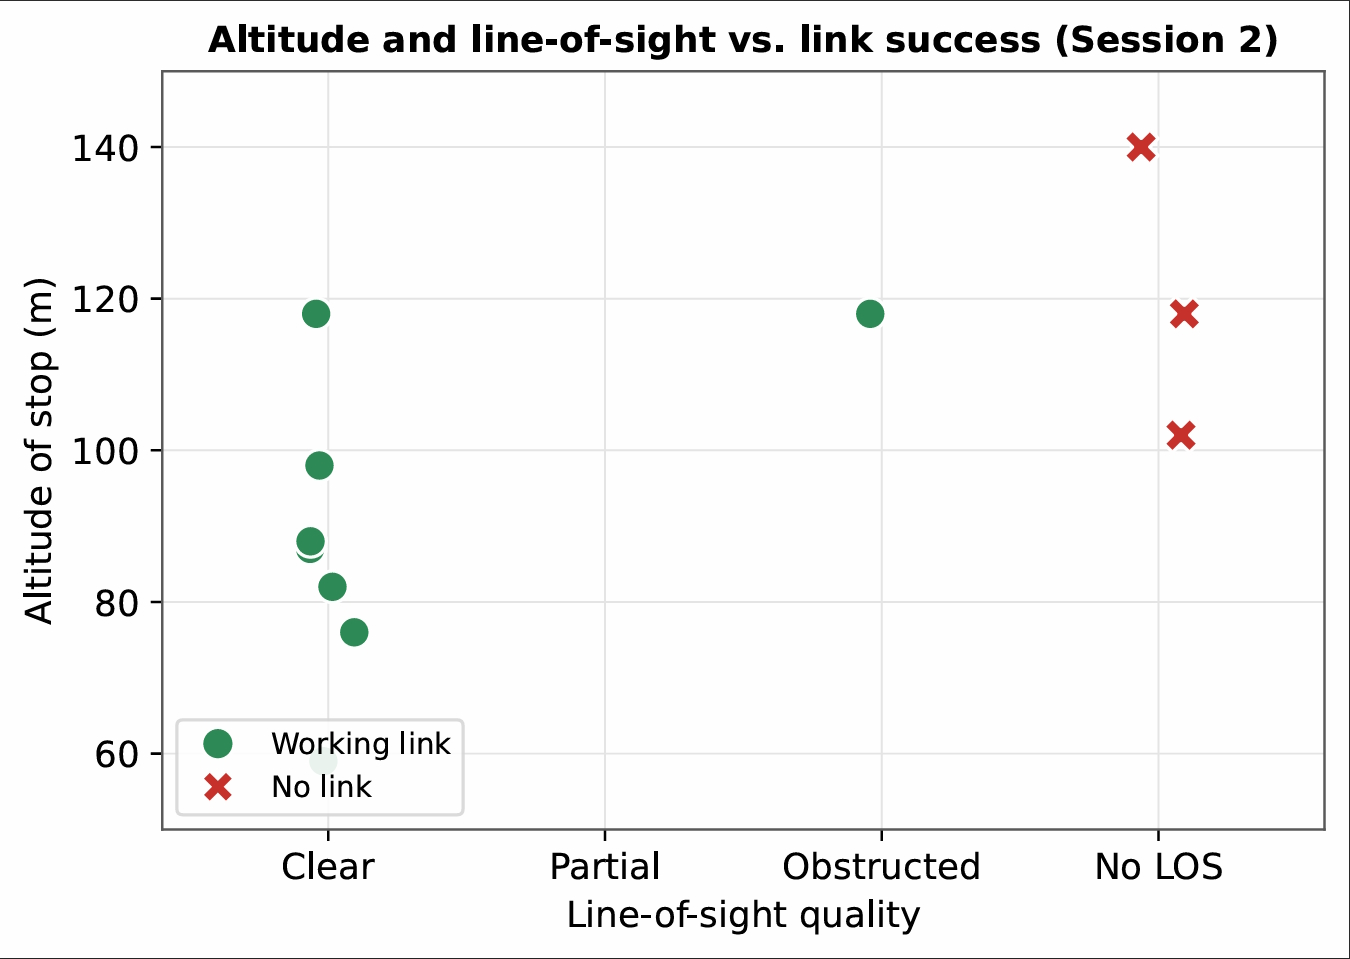
\includegraphics[width=0.85\textwidth]{plot-los-altitude.pdf}
  \caption[Altitude and line-of-sight versus link success (Session~2).]{\label{fig:poc-los}Altitude and \gls{los} quality versus link success in Session~2. The three highest sites (all above 100\,m) failed completely, while lower sites with a clear \gls{los} kept a working link. This confirms that \gls{los} dominates over altitude.}
\end{figure}

As shown in figure~\ref{fig:poc-los}, some sites had good \gls{pdr} and \gls{rssi}, some had good altitude, but none of them combined both succesfully.
The best possibilities from this session were the Malanderpark and Zandstraat tests. But these sites only had a straight line distance of 5.1--5.7\,km to the base node.
On top of this, they didn't have a straightforward mounting point (houses, trees, poles, etc.) so an extra requirement would have been to ask permission to the relevant persons, which was complicated in this situation.
Most of the locations that didn't get any signal were obstructed by surroundings (trees, vegetation, buildings, etc.), this is confirmed by our initial findings during the literature study in section~\ref{sec:sota-lora}.

The Mont-Saint-Aubert possibility stands out as the best option, combining elevation, clear \gls{los} and a person working there who could help with an accessible mounting point.
As seen in Session~1, this location could guarantee a straight-line connection with the base at 18.5\,km.
Permission to mount the relay node was confirmed inside the viewing tower of Floreal Le Panoramique. It offers a clear 180-degree view of the surrounding area, direct access to sunlight, all at a high elevation.
The confirmed location of the relay node were then 50.65457, 3.39975 at an altitude of 140\,m.

Once mounted, the configured relay node was quickly tested to confirm connection with the base node, and communication from mobile to base node through the relay was confirmed.
A next test session was planned to test the effective coverage and limitations of the deployed chain.

\section{Session 3: Deployed-relay coverage mapping}%
\label{sec:poc-session3}

During this third and last test session the base and relay node were set and configured. This session was purely determining the exact coverage and limitations of our current setup.
The mobile node was driven through the south-west/south area of the relay node. This included some locations that were previously marked as ``dead zones''.

Adding a relay node in this connection changed everything, multiple stops achieved a working connection, and the clearest result for this was a confirmed dead zone in Session~1 (50.6133, 3.4128) which was now able to communicate from the mobile node
to the base node passing through the relay node. The connection between the mobile and relay node had a connection with an \gls{rssi} between $-90$ and $-106$\,dBm. The distance between this location and the relay node was only 4.7\,km but no clear \gls{los} was present, the relay node was 140\,m high and the mobile node was at 30\,m.
The distance between the relay and base node was 18.5\,km, which means the total distance travelled by the message was 23.2\,km, straight line distance between the base and mobile node was 19.71\,km.

During this test session the maximum end-to-end distance reached was 30\,km, with a working connection at 11.5\,km from the relay node.
This result was achieved at the ``Rue du préau'' in Taintignies (50.56074, 3.33541) at an altitude of 30\,m. The measurements revealed an \gls{rssi} of $-110$\,dBm and an \gls{snr} of $0.25$\,dB. This means the connection is marginal but still established.

This relay also revealed the effective limitations of Meshtastic using this relay configuration. Locations at low altitude (under 30\,m) at more than 10\,km from the relay were failing to connect. Locations in the city center of Tournai, which is densely built up, also failed.
This means, in our current config the effective range of the relay node was between 10 and 13\,km. If the situation had given us more altitude for the mobile node, a further distance probably could have been achieved.
These findings confirm what was found in the first two test sessions. The obstruction dominates over the altitude, too much obstacles and the connection is impossible or marginal.
In this situation a perfect setup would have been a hill on the opposite side of the city from where the relay is, which would have given more coverage in the city center, and a connection further away, in the flat plains of Wallonia. 

Important to take into account, the shown coverage in this thesis consists of a basic, simple setup with a single relay node without looking for the best optimization possible.
The effective coverage could be improved and extended by placing nodes in higher and less obstructed locations. Replacing the used antennas with higher end (higher gain, directional) antennas such as Yagi or parabolic antennas on the fixed nodes. These antennas would concentrate on a specific axis, which would improve the link but limit the broadcast.
This wasn't the main goal in this thesis as the cost effectiveness was also investigated and we aimed for a wider coverage, this could be changed in function of the goals.
They are, if relevant, a good direction to improve network quality and extend the actual coverage. These are revisited in Chapter~\ref{ch:conclusie}.

The results can be put on a map (figure~\ref{fig:poc-measurements-map}), color-coded by the obtained results:
\begin{figure}[H]
  \centering
  % green = working, orange = marginal, red = failed
  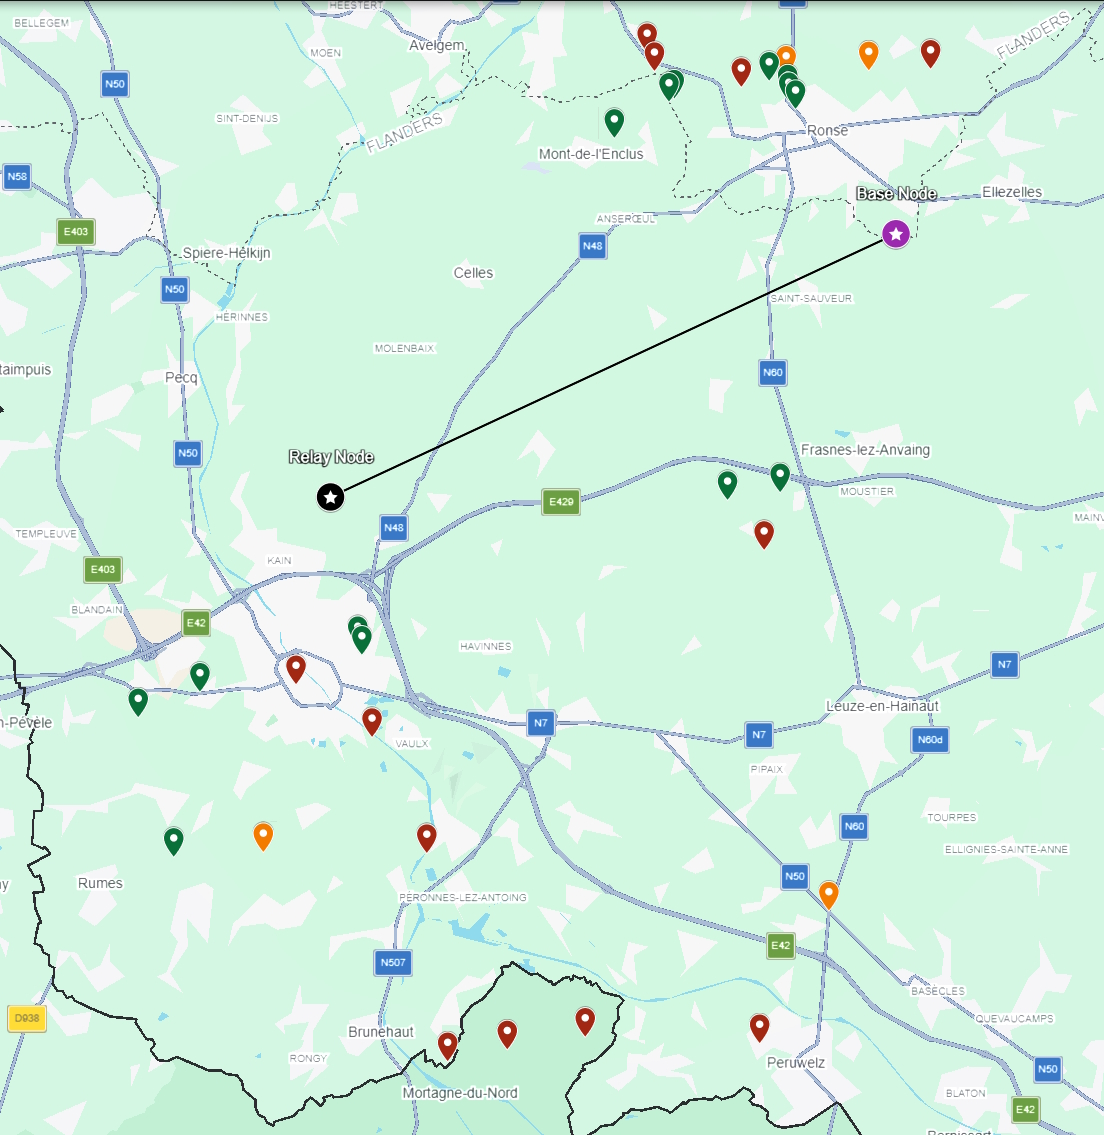
\includegraphics[width=\textwidth]{poc-measurements-map.jpg}
  \caption[Map of all test locations.]{\label{fig:poc-measurements-map}Map of all measurement locations during the tests. Green markers indicate working links, orange markers marginal links, and red markers failed links. The base and relay node are marked separately.}
\end{figure}

\section{Observed mesh participation}%
\label{sec:poc-mesh}

One thing that wasn't expected beforehand is the discovery of other nodes during the setup/tests.
Other devices (Heltec, LilyGo, etc.) configured with the Meshtastic firmware communicated with the deployed nodes, and actively participated in some connections: forwarding messages from mobile to base when the relay was not deployed yet, etc.
This wasn't planned, but it shows exactly what Meshtastic is supposed to do: create a wide network using a Mesh topology to forward messages to areas that might not have the necessary connection.
Some identified nodes reached as far as Amiens, Aalst and Dendermonde, among others.

For example the Amiens node appeared as 2 hops away. The final node (in Amiens) is about 130\,km straight line distance from the base node in Ronse. The Aalst and Dendermonde nodes were closer, at about 40\,km and 50\,km respectively. Both were reached through hops, but these weren't saved to write to this thesis.
This shows that the mesh setup is real, and that the total range of the network is also expandable with good placement of nodes.
Of course, the Amiens node wasn't tested as this was a third-party node, and quite a drive for this \gls{poc}, but it shows the real potential of Meshtastic.

This is the self-organizing nature of Meshtastic. Nodes discover one another and exchange necessary information for routing. This makes the range instantly larger than what you originally expected.
This shows the mesh is a real, practical solution for establishing a connection between distant points. They however could forward the packets, but they couldn't read any content of these packets.
That's the whole point of the secure encryption Meshtastic offers.

\section{Security demonstration}%
\label{sec:poc-security}

The security analysis is mostly done using documentation. Observations can be found in section~\ref{sec:sota-security}.

During the test sessions third-party nodes appeared (as discussed in section \ref{sec:poc-mesh}). At that point our nodes were still running the
default \gls{psk} being \texttt{AQ==}. This means that each node intercepting and forwarding the traffic could decrypt the messages. This is of course not safe, so the \gls{psk} was changed to a random 256-bit key.
This last key was then shared between all three nodes.
The difference is that now the nodes can forward the messages but they can't read them.
Some parts of the packets are not encrypted, and these parts guide the routing of that package (node identifiers, timing, hop count).

This showed one of the main security issues of Meshtastic, when using the default \gls{psk} traffic seems secure but in reality, nothing really is as this default is known by everyone.
Another limitation found is that the \gls{psk} is the same on all three nodes, which means if one of the nodes ``is compromised'' none of the traffic still is secure, also the fact the \gls{psk} is the same
on each node it means the key has to be shared with each participant node, which also involves a security issue.

\section{Autonomous solar operation}%
\label{sec:poc-solar}

In the end, the autonomous operation of said nodes was also evaluated. These nodes having to be deployed during an emergency, we can't ensure the main electrical supply survived.
To avoid any of these issues the test was conducted using a LiPo battery (3.7\,V, 2,000\,mAh) and a 6\,W solar panel (for charging the battery and operation during day time).
This setup was used for both the fixed nodes.

The relay node was set up as ``Power saving'' mode, while the base node was completely set up without any limits, and even WiFi enabled (which consumes even more power).
Theoretically, the battery of 2,000\,mAh and 3.7\,V (storing 7.4\,Wh) should be able to run the setup during 20 to 30 hours. This is calculated using an estimation of 0.3\,W of usage on the setup.
This time is the buffer time before the setup fails.

In reality, what was observed is after a full day of sunlight, the battery took effectively over at night time, the battery level on the base node (with WiFi enabled, so more consumption) was at 75\% by the time it started charging again.
This means that the battery could in reality sustain 4x ±8 hours, which means about 32 hours of total operation. This is a good result, as the battery then charges when sunlight hits it. This means the battery could cover a night + a partially clear sky for example.

In practice the solar panel charges the battery whenever it is hit with sunlight. Telemetry from the V4 reports a full battery and a 4.32\,V voltage, this confirms that during summer the solar panel produces enough energy for charging and operation.
This proves the low-cost combination of a small LiPo battery and a solar panel is enough to keep a node of this size running without any external party being involved.


% Voeg hier je eigen hoofdstukken toe die de ``corpus'' van je bachelorproef
% vormen. De structuur en titels hangen af van je eigen onderzoek. Je kan bv.
% elke fase in je onderzoek in een apart hoofdstuk bespreken.

%\input{...}
%\input{...}
%...

%%=============================================================================
%% Conclusie
%%=============================================================================

\chapter{\IfLanguageName{dutch}{Conclusie}{Conclusion}}%
\label{ch:conclusie}

\section{Answer to the research question}%
\label{sec:conclusion-answer}

This thesis started by investigating to what extent Meshtastic, as a decentralized \gls{lora}-based mesh network, offers a reliable and readily deployable emergency communication solution when primary network infrastructure fails.
Based on the initial literature study and the \gls{poc}, the answer to this question would be yes, on certain conditions.

The \gls{poc} showed that a low-cost Meshtastic setup can provide a real, working link over real distances without relying on any existing infrastructure. A direct connection between two nodes reached a maximum of 18.5\,km, and adding a single relay in this setup improved the end-to-end distance (from Base-Node to mobile node) to 30\,km, which is larger than the literature study suggested.
The \gls{poc} also proved a relay could convert a dead zone connection into a working connection (session 1 compared to session 3). When comparing against the five initial requirements the literature study gave us in chapter~\ref{ch:stand-van-zaken}, Meshtastic can be seen as a realistic alternative.
It performs well on infrastructure independence, deployability and affordability, and for security, while it has limitations, it offers a reasonable level of protection if correctly configured.
These figures come from three sessions in a single region with one hardware type, so they should be read as an indication rather than a guaranteed performance benchmark.

For the problem domain, the identified gaps were solutions that don't depend on main infrastructure, which are quick to deploy and are affordable at scale. Both \gls{aprs} and \gls{dmr} fail because of the licensing requirements. Satellite messengers like Garmin inReach and Zoleo mainly fail because of the recurring costs.
Meshtastic is the only alternative that ticks every box. Regarding the environmental factors, the \gls{poc} showed us that the trees, buildings and other obstructions impede the signal way more than just the distance or the altitude.
This was clearly illustrated in section~\ref{sec:poc-session2} where the highest test locations (Hotond, Kwaremont) had 0\,\% \gls{pdr} because of the trees, while lower altitude locations but with a clear \gls{los} achieved 100\,\%.
The security question is a bit tricky on Meshtastic. The messages are effectively encrypted using \gls{aes}-256 once a private key is configured, but the default channel is public, so on a wrong config every message isn't really encrypted. Also once set up, the channels don't use authentication to make sure the message is from the right device.
If someone gets the key, they can impersonate a node and send messages on the channel. The header of the message is also in cleartext, so the metadata is not protected. The private communication between devices (end-to-end, no channel usage) is protected by encryption and, unlike the shared channels, also by authentication.

The range and reliability question from the solution domain has also been answered in the \gls{poc}.
The maximum direct connection distance achieved between two nodes was 18.5\,km, and with a single relay, the end-to-end distance was 30\,km. The effective range of the relay was estimated at 10 to 13\,km depending on terrain.
On the security question, just as mentioned before, confidentiality holds up, but authentication and metadata protection do not. This has also been discussed in section~\ref{sec:poc-security}.

Compared to the other alternatives, Meshtastic is the only one that combines infrastructure independence, no licence requirement, affordability at scale and low-barrier deployment. The current setup is easy to set up and understand, but needs some technical know-how to install (section~\ref{sec:poc-config}).

\section{Reflection}%
\label{sec:conclusion-reflection}

The effective total range of a clear \gls{los} connection was surprising going into the \gls{poc}. The assumption was that the higher the node, the better the connection. But the results showed that a lower location with a better \gls{los} outperforms most high altitude nodes surrounded by trees.
This is important for a real-world deployment: picking a relay location isn't just ``find the highest point'', but it's ``finding the point with the best \gls{los} in the direction you need coverage''.

Something that makes sense, but wasn't expected either was the discovery of third-party nodes during testing, some as far as Amiens, roughly 130\,km away.
This was as said unexpected, but it was convincing that the mesh topology is actually working as intended: nodes that weren't configured together still find a way to route traffic between them.

While Meshtastic is cheap and doesn't need a licence, which checks the deployability box on paper, the difficulties encountered during the setup in section~\ref{sec:poc-config} show that some patience, and a basic technical knowledge is necessary (CLI config if web client unreliable, etc.).

\section{Limitations}%
\label{sec:conclusion-limitations}

Some limitations were also discovered. The only tested hardware was the Heltec WiFi LoRa 32 V4; \gls{aprs}, \gls{dmr}, satellite messengers were only evaluated through literature study. Also other ESP32 options exist but weren't tested. They should work in the same way this \gls{poc} was done.
The comparison combines measured data on one side with documented data on the other. All measurements were also done in a single region (around Ronse and Tournai) and during a dry summer period. The results may look different in a more flat region, or during winter time, etc.
Latency, which was listed as a metric in the original proposal, was intentionally left out of the measured scope (see section~\ref{sec:method-measurement}). It was just informally noted, seeing traceroutes and messages arrived within a few seconds, which is good enough for this kind of scenarios.
Range and packet delivery turned out to be the decisive factors for answering the research question.
As planned, the security analysis stayed documentation-based combined with some setup observations. No real traffic has been intercepted or decrypted, both because that would be illegal and because it fell outside the scope of this thesis.

\section{Future research}%
\label{sec:conclusion-future}

The most obvious next step for continuing this research is to expand the \gls{poc} with more nodes, and more relays. This would allow to test even more hops and see how far the range could be extended using more nodes.
Each node probably adds some packet loss. It would be useful to know exactly how much and how far (in terms of hops and distance) this type of network can be pushed before it stops being useful.

A rough estimation can be made on creating a longer multi-hop path. The first hop of the current setup (base to relay) reached 18.5\,km with a clear \gls{los}. The second hop (relay to mobile) reached an effective 10--13\,km, which gave us a 30\,km end-to-end distance.
If a second relay would be added at another elevated, clear-\gls{los} site, a comparable third hop of roughly 10--15\,km could be estimated. This would extend the theoretical reach of the chain to approximately 45--50\,km over three hops.
This remains an estimation; every additional hop adds latency and more chance of packet loss. If a second relay would be introduced, the hop limit setting should also be moved from 3 to a higher count.
An effective test with a second relay should be done to confirm the effective range. That's a clear direction for further research.

Another next step could be testing in different environmental conditions. This was supposed to be done during the \gls{poc}, but the weather stayed largely dry and calm throughout the \gls{poc} (20 July 2026 – 20 August 2026),
so no systematic weather comparison was possible during the sessions. Only one day allowed testing in the rain (section~\ref{sec:poc-rain}).
This does not mean the setup is viable in all weather conditions, but it shows that rain does not necessarily break the connection, and this should be confirmed in future research.
The same measurements could be repeated but at different times of the day, and most importantly, in different weather conditions (rain, wind, temperature swings) to see whether the change in conditions has a real-world effect on the stability of the connection.

Going more into the security side of Meshtastic could be another direction to dig into, especially authentication and metadata protection (section~\ref{sec:sota-security}).
Lastly, as mentioned in section~\ref{sec:poc-session3}, using higher-gain or directional antennas (such as Yagi, parabolic, etc.) instead of a small omnidirectional one could largely improve the quality and the range of the network. The broadcast aspect would likely be lost, but in return the range and quality could be extended.
This wasn't tested during this thesis due to cost and time constraints, but it is a realistic next step for anyone trying to push the research even further.


\section{Comparison matrix}%
\label{sec:conclusion-comparison}
\begin{table}[H]
  \centering
  \begin{tabular}{lcccc}
    \toprule
    \textbf{Requirement} & \textbf{APRS} & \textbf{DMR} & \textbf{Satellite} & \textbf{Meshtastic} \\
    \midrule
    Infrastructure-independent   & Yes     & Partial & Yes    & Yes             \\
    Low-barrier deployment       & No      & No      & Yes    & Yes             \\
    Affordable at scale          & Partial & Partial & No     & Yes             \\
    No licence required          & No      & No      & Yes    & Yes             \\
    Range and reliability        & Good    & Good    & Global & Good            \\
    \midrule
    Data throughput              & Low     & High    & Low    & Very low        \\
    Message type                 & Text    & Voice + data & Text & Text + telemetry \\
    Guaranteed delivery          & No      & Yes     & Yes    & No (best-effort) \\
    Independent of node density  & Yes     & Yes     & Yes    & No              \\
    \bottomrule
  \end{tabular}
  \caption[Comparison of off-grid communication alternatives.]{\label{tab:conclusion-comparison}Comparison of the reviewed off-grid communication alternatives.}
\end{table}

The completed matrix and conclusion confirms that Meshtastic is not a universal winner.
It trades throughput, voice capability and guaranteed delivery for cost, licence-free use and easy deployment requirements.
For the specific scenario of this thesis, a low-cost text-based network that survives infrastructure failure, that trade-off is favourable, but it would be a poor choice where high bandwidth, voice, or guaranteed delivery are required.

\section{Recommendations for practitioners}%
\label{sec:conclusion-recommendations}

After a \gls{poc} like this, anyone considering Meshtastic for a real emergency deployment should take some practical points into account.
First, node placement should be planned around \gls{los}, not just around altitude.
Second, \textbf{always} replace the default encryption key with a random private key before using the network for anything sensitive, using the default key is basically the same as not encrypting any of the traffic at all.
Third, if main power isn't guaranteed, the nodes can easily run on a solar panel and battery (with the battery taking over at nighttime). In this \gls{poc} this was tested with a combination of a 6\,W, 5\,V/1.2\,A solar panel and a 3.7\,V, 2,000\,mAh battery. These could also be upgraded to a larger panel and battery if needed, but this setup was more than enough to run a node continuously through the night.
Both the solar powered nodes have been powered during a month without having to intervene.
Finally, the web interface not always being reliable during the setup, the mobile app or the command-line interface should be used for configuration instead.

With these points taken into account, Meshtastic stays a genuinely usable, low-cost option for emergency communication, well within the reach of volunteer organisations or small teams without a big budget or specialized licences.

%---------- Bijlagen -----------------------------------------------------------

\appendix

\chapter{Thesis proposal}

The subject of this bachelor thesis is based on a research proposal that was previously reviewed by the supervisor. That proposal is included in this appendix.

%% TODO: 
%\section*{Samenvatting}

% Kopieer en plak hier de samenvatting (abstract) van je onderzoeksvoorstel.

% Verwijzing naar het bestand met de inhoud van het onderzoeksvoorstel
%---------- Inleiding ---------------------------------------------------------

% TODO: Is dit voorstel gebaseerd op een paper van Research Methods die je
% vorig jaar hebt ingediend? Heb je daarbij eventueel samengewerkt met een
% andere student?
% Zo ja, haal dan de tekst hieronder uit commentaar en pas aan.

%\paragraph{Opmerking}

% Dit voorstel is gebaseerd op het onderzoeksvoorstel dat werd geschreven in het
% kader van het vak Research Methods dat ik (vorig/dit) academiejaar heb
% uitgewerkt (met medesturent VOORNAAM NAAM als mede-auteur).
% 

\section{Introduction}%
\label{sec:introduction}

Morden society relies heavily (if not entirely) on available communication networks.
This means emergency reponse relies on this as well. When a major storm destroys a cellular
tower, or flooding cuts power, or large-scale incidents overloads the general public channels,
they become unavailable. Or as we've seen recently during wars and communication lines get
intentionally cut off. The moment they become unavailable, is the exact moment they are needed
the most. In those scenarios first responders, civil protection services and communities need a
fallback that is independent of the existing fixed infrastructure. For those situations this
should be easily and fast deployable solution, without needing any specialist and it
should also be afordable at scale.

A few off-the-grid communication technologies already exist, but they all have their own limitions
in emergency contexts. \textbf{APRS} (Automatic Packet Reporting System) and \textbf{DMR}
(Digital Mobile Radio) both require an amateur radio license and special equiment (specialized hardware
configuration). This makes them hard to deploy in emergency situations. Commercial satellite messengers
and phones (e.g. Garmin inReach or SPOT) are expensive and they require a subscription cost, plus per-message
fees. These limitations make large-scale deployments nearly impossible for small volunteer or
municipal emergency organizations. However, on the other side of the spectrum we also have mesh
radio networks, which are built on \textbf{LoRa} (Long Range) radio technology.
They represent a totally different approach, they are low-power, license-free operating
devices in the \emph{sub-GHz ISM band}, using multi-hop routing which will then extend our coverage
without needing any fixed infrastructure.

To do this we can be looking at \textbf{Meshtastic}.
First, what is Meshtastic?
\begin{itemize}
  \item Open-source firmware and protocol stack for LoRa-capable microcontrollers (mostly ESP32)
  \item Encrypted and decentralized text messaging, locatrion sharing
  \item Self-healing mesh network, multi-hop routing
  \item No need of a SIM card or internet connection, no license
\end{itemize}
Why Meshtastic? On top of the previous mentioned advantages, anecdotes form community deployments and disaster
response suggest promising results. However, no scientific, systematic, empirical research has been done on the
reliability, deployability and evalution of it's performance in emergency situations has yet been published.
This gap in research motivates the following research question:
\textbf{To what extent does Meshtastic, as a decentralized LoRa-based mesh network, offer a reliable and readily deployable emergency communication solution when primary network infrastructure fails?}

\subsection{Problem Domain}%
\label{subsec:problem-domain}
Let's examine and evaluate thje communication requirements that come up when the primary infrastructure fails, and if there are any adequate solutions to fix them.
Three sub-questions guide us:
\begin{itemize}
  \item What gaps exist in emergency contexts when the primary infra becomes unavailable?
  \item How do exisitng alternatives compare to Meshtastioc in terms of accessibility, cost, required expertise, etc. ?
  \item What environmental factors of the Belgian landscape and terrain affect LoRa performances once deployed.
  \item How secure is the Meshtastic encrytion in case of traffic interception?
\end{itemize}

\subsection{Solution Domain}%
\label{subsec:solution-domain}
What are the actual performances of a Meshtastic setup, evaulated through a structured PoC and compare those results.
Three sub-questions emerge here as well:
\begin{itemize}
  \item What range and reliability does a Meshtastic network have across different topologies (direct long-distance
  vs multi-hop network) in a real deployment (East Flanders province)?
  \item How does the Meshtastic security model hold up against potential attacks?
  \item How does it compare with other alternatives in terms of requirements in emergency situations?
\end{itemize}

\subsection{Target audience and scope}%
\label{subsec:target-audience-and-scope}
The main audience are IT professionals responsible for business continuity planning and civil protection communication
in case of emergencies. A secondary audience we could describe are volunteer organizations, municipal safety services and 
network enginess evaluating low-cost off the gris communication options, to be independent of the main societal infrastructure.

The scope of our research is limited by following constraints.
\begin{itemize}
  \item The hardware testing stays limited to Meshtastic due to budget and time constraitns. Alternatives will be evaultaed using litterature only.
  \item The PoC setup and measurtements will onlu be on the EU\_868MHz freqeuncy, this is dictated by \textbf{BIPT} (Belgisch Instituut voor Postdiensten en Telecommunicatie).
\end{itemize}
The geographical focus of the PoC will be the East-Flanders province. Measurements will be taken on the
the direct long-distance link between Ronse and Lochristi (Ghent), this straight connection will cover ~65km.
This is most-definitely unfeasible as a direct LoRa link. That's why we will evalute a multi-hop chain, with nodes in Oudenaarde and maybe Marelbeke (if necessary).
These different setups and measuremnts will help us achieve meaningful results about the reliabiltiy, and limitions of Meshtastic on longer distances.

%---------- Stand van zaken ---------------------------------------------------

\section{Literatuurstudie}%
\label{sec:literatuurstudie}

Hier beschrijf je de \emph{state-of-the-art} rondom je gekozen onderzoeksdomein, d.w.z.\ een inleidende, doorlopende tekst over het onderzoeksdomein van je bachelorproef. Je steunt daarbij heel sterk op de professionele \emph{vakliteratuur}, en niet zozeer op populariserende teksten voor een breed publiek. Wat is de huidige stand van zaken in dit domein, en wat zijn nog eventuele open vragen (die misschien de aanleiding waren tot je onderzoeksvraag!)?

Je mag de titel van deze sectie ook aanpassen (literatuurstudie, stand van zaken, enz.). Zijn er al gelijkaardige onderzoeken gevoerd? Wat concluderen ze? Wat is het verschil met jouw onderzoek?

Verwijs bij elke introductie van een term of bewering over het domein naar de vakliteratuur, bijvoorbeeld~\autocite{Hykes2013}! Denk zeker goed na welke werken je refereert en waarom.

Draag zorg voor correcte literatuurverwijzingen! Een bronvermelding hoort thuis \emph{binnen} de zin waar je je op die bron baseert, dus niet er buiten! Maak meteen een verwijzing als je gebruik maakt van een bron. Doe dit dus \emph{niet} aan het einde van een lange paragraaf. Baseer nooit teveel aansluitende tekst op eenzelfde bron.

Als je informatie over bronnen verzamelt in JabRef, zorg er dan voor dat alle nodige info aanwezig is om de bron terug te vinden (zoals uitvoerig besproken in de lessen Research Methods).

% Voor literatuurverwijzingen zijn er twee belangrijke commando's:
% \autocite{KEY} => (Auteur, jaartal) Gebruik dit als de naam van de auteur
%   geen onderdeel is van de zin.
% \textcite{KEY} => Auteur (jaartal)  Gebruik dit als de auteursnaam wel een
%   functie heeft in de zin (bv. ``Uit onderzoek door Doll & Hill (1954) bleek
%   ...'')

Je mag deze sectie nog verder onderverdelen in subsecties als dit de structuur van de tekst kan verduidelijken.

%---------- Methodologie ------------------------------------------------------
\section{Methodologie}%
\label{sec:methodologie}

Hier beschrijf je hoe je van plan bent het onderzoek te voeren. Welke onderzoekstechniek ga je toepassen om elk van je onderzoeksvragen te beantwoorden? Gebruik je hiervoor literatuurstudie, interviews met belanghebbenden (bv.~voor requirements-analyse), experimenten, simulaties, vergelijkende studie, risico-analyse, PoC, \ldots?

Valt je onderwerp onder één van de typische soorten bachelorproeven die besproken zijn in de lessen Research Methods (bv.\ vergelijkende studie of risico-analyse)? Zorg er dan ook voor dat we duidelijk de verschillende stappen terug vinden die we verwachten in dit soort onderzoek!

Vermijd onderzoekstechnieken die geen objectieve, meetbare resultaten kunnen opleveren. Enquêtes, bijvoorbeeld, zijn voor een bachelorproef informatica meestal \textbf{niet geschikt}. De antwoorden zijn eerder meningen dan feiten en in de praktijk blijkt het ook bijzonder moeilijk om voldoende respondenten te vinden. Studenten die een enquête willen voeren, hebben meestal ook geen goede definitie van de populatie, waardoor ook niet kan aangetoond worden dat eventuele resultaten representatief zijn.

Uit dit onderdeel moet duidelijk naar voor komen dat je bachelorproef ook technisch voldoen\-de diepgang zal bevatten. Het zou niet kloppen als een bachelorproef informatica ook door bv.\ een student marketing zou kunnen uitgevoerd worden.

Je beschrijft ook al welke tools (hardware, software, diensten, \ldots) je denkt hiervoor te gebruiken of te ontwikkelen.

Probeer ook een tijdschatting te maken. Hoe lang zal je met elke fase van je onderzoek bezig zijn en wat zijn de concrete \emph{deliverables} in elke fase?

%---------- Verwachte resultaten ----------------------------------------------
\section{Verwacht resultaat, conclusie}%
\label{sec:verwachte_resultaten}

Hier beschrijf je welke resultaten je verwacht. Als je metingen en simulaties uitvoert, kan je hier al mock-ups maken van de grafieken samen met de verwachte conclusies. Benoem zeker al je assen en de onderdelen van de grafiek die je gaat gebruiken. Dit zorgt ervoor dat je concreet weet welk soort data je moet verzamelen en hoe je die moet meten.

Wat heeft de doelgroep van je onderzoek aan het resultaat? Op welke manier zorgt jouw bachelorproef voor een meerwaarde?

Hier beschrijf je wat je verwacht uit je onderzoek, met de motivatie waarom. Het is \textbf{niet} erg indien uit je onderzoek andere resultaten en conclusies vloeien dan dat je hier beschrijft: het is dan juist interessant om te onderzoeken waarom jouw hypothesen niet overeenkomen met de resultaten.



%%---------- Andere bijlagen --------------------------------------------------
\chapter{Node configuration reference}%
\label{ch:bijlage-config}

This appendix lists the full configuration of the three deployed nodes as a technical
reference, complementing the summary given in Table~\ref{tab:poc-config}. Values were
read out using the Meshtastic command-line interface (\texttt{--info}) after the final
configuration of each node.
Quick note: WiFi doesn't need to be enabled, but with the node on the roof, this was easier to access the rangetest csv file.

\section{Radio and device configuration}%
\label{sec:bijlage-config-device}

\begin{table}[h]
  \centering
  \small
  \begin{tabular}{lccc}
    \toprule
    \textbf{Parameter} & \textbf{Ronse-Base} & \textbf{Relay} & \textbf{Mobile} \\
    \midrule
    Role                    & CLIENT\_BASE & ROUTER      & CLIENT \\
    Firmware                & 2.7.26.54e0d8d & 2.7.26.54e0d8d & 2.7.26.54e0d8d \\
    Hardware model          & Heltec V4    & Heltec V4   & Heltec V4 \\
    Region                  & EU\_868      & EU\_868     & EU\_868 \\
    Modem preset            & LONG\_FAST   & LONG\_FAST  & LONG\_FAST \\
    Bandwidth               & 250\,kHz     & 250\,kHz    & 250\,kHz \\
    Spreading factor        & 11           & 11          & 11 \\
    Coding rate             & 4/5          & 4/5         & 4/5 \\
    Hop limit               & 3            & 3           & 3 \\
    TX power                & 27\,dBm      & 27\,dBm     & 27\,dBm \\
    Boosted RX gain         & Enabled      & Enabled     & Enabled \\
    FEM/LNA mode            & Disabled     & Disabled    & Disabled \\
    Rebroadcast mode        & ALL          & ALL         & ALL \\
    \midrule
    Fixed position          & Yes          & Yes         & No (GPS via phone) \\
    Latitude                & 50.72316     & 50.65457    & --- \\
    Longitude               & 3.63217      & 3.39975     & --- \\
    Altitude                & 90\,m        & 140\,m      & --- \\
    \midrule
    Power saving            & Off          & On          & Off \\
    Bluetooth                & Enabled, no PIN & Enabled, no PIN & Enabled, no PIN \\
    WiFi                     & Enabled (bridge) & Disabled & Disabled \\
    Display screen timeout   & 60\,s        & 30\,s       & 60\,s \\
    \bottomrule
  \end{tabular}
  \caption[Radio and device configuration]{\label{tab:bijlage-config}Radio and device configuration of the three nodes.}
\end{table}

\section{Module configuration}%
\label{sec:bijlage-config-modules}

On top of the default settings, Meshtastic exposes a number of independent modules
that were configured per node according to its role. Table~\ref{tab:bijlage-modules}
lists the modules relevant to this deployment; modules not used in this thesis
(such as Store\&Forward, Detection Sensor, Paxcounter, Audio and Canned Message)
were left at their firmware defaults (disabled) on all nodes.

\begin{table}[h]
  \centering
  \small
  \begin{tabular}{lccc}
    \toprule
    \textbf{Module} & \textbf{Ronse-Base} & \textbf{Relay} & \textbf{Mobile} \\
    \midrule
    \multicolumn{4}{l}{\textit{Range Test}} \\
    Enabled                 & Yes (receiver) & Yes (receiver) & Yes (sender) \\
    Sender interval         & ---          & ---         & 60\,s \\
    CSV logging             & Enabled      & Disabled    & --- \\
    \midrule
    \multicolumn{4}{l}{\textit{Telemetry}} \\
    Device telemetry        & Enabled      & Enabled     & Enabled \\
    Update interval         & 1,800\,s      & 1,800\,s     & 1,800\,s \\
    Environment telemetry   & Disabled     & Disabled    & Disabled \\
    \midrule
    \multicolumn{4}{l}{\textit{Neighbor Info}} \\
    Enabled                 & Yes          & Yes         & Yes \\
    Update interval         & 21,600\,s      & 21,600\,s     & 21,600\,s \\
    \midrule
    \multicolumn{4}{l}{\textit{MQTT}} \\
    Enabled                 & No           & No          & No \\
    \bottomrule
  \end{tabular}
  \caption[Module configuration]{\label{tab:bijlage-modules}Module configuration of the three deployed nodes.}
\end{table}

\section{Channel and security configuration}%
\label{sec:bijlage-config-security}

All three nodes were migrated from the Meshtastic default public channel to a private
channel secured with a randomly generated 256-bit \gls{psk}, as discussed in
Section~\ref{sec:poc-security}. The channel name and \gls{psk} are identical across all three
nodes so that they can communicate; the \gls{psk} itself is not reproduced here for obvious
reasons.

\begin{table}[h]
  \centering
  \small
  \begin{tabular}{ll}
    \toprule
    \textbf{Parameter} & \textbf{Value} \\
    \midrule
    Channel index         & 0 (primary) \\
    PSK type              & Random, 256-bit \\
    PSK identical across nodes & Yes (verified via channel URL) \\
    Uplink/downlink enabled & No \\
    \bottomrule
  \end{tabular}
  \caption[Channel security configuration]{\label{tab:bijlage-security}Channel security configuration, identical on all three nodes.}
\end{table}
\chapter{Rangetest logs}%
\label{ch:bijlage-rangetest}

This appendix shows a small part of the rangetest logs. The full raw data file can be found in the repository.
The rangetest module was performed across all three sessions, and was actively used to determine the coverage and best relay locations. The logs contain the following fields:
\begin{itemize}
    \item \textbf{time}: timestamp of the log entry
    \item \textbf{from}: sender ID of the message
    \item \textbf{sender name}: name of the sender node
    \item \textbf{sender lat}: latitude of the sender
    \item \textbf{sender long}: longitude of the sender
    \item \textbf{rx lat}: latitude of the receiving node
    \item \textbf{rx long}: longitude of the receiving node
    \item \textbf{rx elevation}: the elevation of the receiving node
    \item \textbf{rx snr}: the signal-to-noise ratio at the receiving node
    \item \textbf{distance}: the distance between sender and receiver in meters
    \item \textbf{hop limit}: the hop limit for this message
    \item \textbf{payload}: any additional payload data sent with this message
    \item \textbf{rx rssi}: the received signal strength indicator at the receiving node
    \item \textbf{seq}: the sequence number of the message
\end{itemize}

\begin{listing}[H]
  \begin{minted}{text}
    time,from,sender name,sender lat,sender long,rx lat,rx long,rx elevation,rx snr,distance,hop limit,payload,rx rssi,seq
    00:00:12,-1884870688,,0.000000,0.000000,50.723060,3.632340,88,-6.500000,0,0,"seq 2"
    -116,06:28:32,-1884870688,,0.000000,0.000000,50.723060,3.632340,88,-10.000000,0,0,"seq 3"
    -120,06:29:32,-1884870688,,0.000000,0.000000,50.723060,3.632340,88,-8.250000,0,0,"seq 4"
    -118,06:30:32,-1884870688,,0.000000,0.000000,50.723060,3.632340,88,-4.500000,0,0,"seq 5"
    -114,06:31:32,-1884870688,,0.000000,0.000000,50.723060,3.632340,88,-4.250000,0,0,"seq 6"
    -114,06:32:32,-1884870688,,0.000000,0.000000,50.723060,3.632340,88,-17.500000,0,0,"seq 7"
    -127,06:33:32,-1884870688,,0.000000,0.000000,50.723060,3.632340,88,-16.250000,0,0,"seq 8"
    -126,06:34:32,-1884870688,,0.000000,0.000000,50.723060,3.632340,88,-11.250000,0,0,"seq 9"
    -121,06:35:32,-1884870688,,0.000000,0.000000,50.723060,3.632340,88,-14.000000,0,0,"seq 10"
    -123,06:37:33,-1884870688,,0.000000,0.000000,50.723060,3.632340,88,-12.750000,0,0,"seq 12"
    -123,06:38:33,-1884870688,,0.000000,0.000000,50.723060,3.632340,88,-12.500000,0,0,"seq 13"
    -122,06:39:33,-1884870688,,0.000000,0.000000,50.723060,3.632340,88,-15.250000,0,0,"seq 14"
    -125,06:40:33,-1884870688,,0.000000,0.000000,50.723060,3.632340,88,-12.250000,0,0,"seq 15"
    -122,06:41:33,-1884870688,,0.000000,0.000000,50.723060,3.632340,88,-12.000000,0,0,"seq 16"
    -122,06:42:33,-1884870688,,0.000000,0.000000,50.723060,3.632340,88,-11.250000,0,0,"seq 17"
    -121,06:43:33,-1884870688,Mobile,0.000000,0.000000,50.723060,3.632340,88,-8.750000,0,0,"seq 18"
    -119,06:44:33,-1884870688,Mobile,0.000000,0.000000,50.723060,3.632340,88,-14.750000,0,0,"seq 19"
    -124,06:46:33,-1884870688,Mobile,0.000000,0.000000,50.723060,3.632340,88,5.000000,0,0,"seq 21"
    -101,06:47:34,-1884870688,Mobile,0.000000,0.000000,50.723060,3.632340,88,4.250000,0,0,"seq 22"
    -100,06:48:34,-1884870688,Mobile,0.000000,0.000000,50.723060,3.632340,88,5.750000,0,0,"seq 23"
    -102,06:49:34,-1884870688,Mobile,0.000000,0.000000,50.723060,3.632340,88,5.750000,0,0,"seq 24"
    -101,06:50:34,-1884870688,Mobile,0.000000,0.000000,50.723060,3.632340,88,5.500000,0,0,"seq 25"
    -101,06:54:34,-1884870688,Mobile,0.000000,0.000000,50.723060,3.632340,88,0.000000,0,0,"seq 29"
    -111,06:55:34,-1884870688,Mobile,0.000000,0.000000,50.723060,3.632340,88,-0.250000,0,0,"seq 30"
    -111,06:56:34,-1884870688,Mobile,0.000000,0.000000,50.723060,3.632340,88,-12.000000,0,0,"seq 31"
    -122,06:58:34,-1884870688,Mobile,0.000000,0.000000,50.723060,3.632340,88,-10.500000,0,0,"seq 33"
    -120,06:59:34,-1884870688,Mobile,0.000000,0.000000,50.723060,3.632340,88,6.000000,0,0,"seq 34"
    -77,07:00:34,-1884870688,Mobile,0.000000,0.000000,50.723060,3.632340,88,5.750000,0,0,"seq 35"
    -77,07:01:34,-1884870688,Mobile,0.000000,0.000000,50.723060,3.632340,88,6.000000,0,0,"seq 36"
    -75,07:02:35,-1884870688,Mobile,0.000000,0.000000,50.723060,3.632340,88,6.250000,0,0,"seq 37"
    -72,07:03:35,-1884870688,Mobile,0.000000,0.000000,50.723060,3.632340,88,6.500000,0,0,"seq 38"
    -81,07:04:35,-1884870688,Mobile,0.000000,0.000000,50.723060,3.632340,88,-12.750000,0,0,"seq 39"
    -123,07:05:35,-1884870688,Mobile,0.000000,0.000000,50.723060,3.632340,88,5.750000,0,0,"seq 40"
    -74,07:06:35,-1884870688,Mobile,0.000000,0.000000,50.723060,3.632340,88,6.000000,0,0,"seq 41"
    -73,07:07:36,-1884870688,Mobile,0.000000,0.000000,50.723060,3.632340,88,6.000000,0,0,"seq 42"
    -72,07:08:35,-1884870688,Mobile,0.000000,0.000000,50.723060,3.632340,88,6.250000,0,0,"seq 43"
    -70,07:09:35,-1884870688,Mobile,0.000000,0.000000,50.723060,3.632340,88,6.250000,0,0,"seq 44"
    -72,07:10:35,-1884870688,Mobile,0.000000,0.000000,50.723060,3.632340,88,6.000000,0,0,"seq 45"
    -75,07:11:36,-1884870688,Mobile,0.000000,0.000000,50.723060,3.632340,88,7.000000,0,0,"seq 46"
    -74,07:12:36,-1884870688,Mobile,0.000000,0.000000,50.723060,3.632340,88,7.750000,0,0,"seq 47"
    -74,07:13:36,-1884870688,Mobile,0.000000,0.000000,50.723060,3.632340,88,6.250000,0,0,"seq 48"
    -75,07:14:36,-1884870688,Mobile,0.000000,0.000000,50.723060,3.632340,88,6.000000,0,0,"seq 49"
    -74,07:15:36,-1884870688,Mobile,0.000000,0.000000,50.723060,3.632340,88,6.250000,0,0,"seq 50"
  \end{minted}
  \caption[Rangetest log]{Sample of the rangetest log.}
\end{listing}
\chapter{Field measurement logs}%
\label{ch:bijlage-veldnotities}

This appendix contains field notes recorded during Session~2 (relay-candidate
survey) and Session~3 (deployed-relay coverage mapping), complementing the summarized
results in Sections~\ref{sec:poc-session2} and~\ref{sec:poc-session3}. Coordinates,
timestamps and signal readings were recorded on site and standardized below for
readability; raw notes are available in the project repository.

\section{Session 2 -- relay-candidate survey}%
\label{sec:bijlage-session2}

\begin{table}[h]
  \centering
  \tiny
  \begin{tabular}{lccccll}
    \toprule
    \textbf{Location} & \textbf{Alt.\ (m)} & \textbf{Time} & \textbf{RSSI} & \textbf{SNR} & \textbf{LOS} & \textbf{Mountable} \\
    \midrule
    Kruisstraat (low)    & 56  & 11:23--11:29 & $-103$\,dBm & $+3.75$\,dB  & Direct/almost      & Possibly (housing) \\
    Kruisstraat (high)   & 74  & 11:30--11:36 & $-110$\,dBm & $-0.75$\,dB  & Direct/almost      & Possibly (housing) \\
    Kruisstraat (top)    & 117 & 11:37--11:43 & $-122$\,dBm & $-11.0$\,dB  & No, trees/houses   & Possibly (housing) \\
    Zandstraat            & 116 & 11:43--11:48 & $-107$ to $-122$\,dBm & $-2.75$ to $-11.5$\,dB & Almost, few trees & Guardrail, clear view \\
    Hotond (top)          & 138 & 11:49--11:55 & No response & No response  & No, trees          & Café Hotond (unconfirmed) \\
    Kwaremont (top)       & 100 & ---           & No response & No response  & No, trees          & Trees/houses only \\
    Knokte / Trieu (top)  & 116 & ---           & No response & No response  & No, trees          & Trees/houses only \\
    Karnemelkbeekstraat   & 80  & 12:12--12:18 & $-106$\,dBm & $+2.75$\,dB  & Clear              & Unclear (house/trees) \\
    Drie Lindenstraat     & 88  & 12:19--12:23 & $-109$\,dBm & $+0.75$\,dB  & Clear/almost       & Fields, bench, trees \\
    Malanderpark (foot)   & 98  & 12:30--12:40 & $-106$ to $-110$\,dBm & $+0.5$ to $+3.75$\,dB & Almost clear & Park (trees) \\
    Ten Bergestraat       & 86  & 12:52--12:55 & $-118$\,dBm & $-6.75$\,dB  & Clear/almost       & Houses \\
    Muziekbos/Kanarieberg & 148 & ---           & No signal   & No signal    & ---                & Not usable, no data recorded \\
    \bottomrule
  \end{tabular}
  \caption[Session 2]{\label{tab:bijlage-session2}Field log for session 2 (finding an appropriate spot for relay)}
\end{table}

\section{Session 3 -- deployed-relay coverage mapping}%
\label{sec:bijlage-session3}

\begin{table}[h]
  \centering
  \tiny
  \begin{tabular}{cccccccl}
    \toprule
    \textbf{Stop} & \textbf{Alt.\ (m)} & \textbf{Arrival} & \textbf{RSSI (relay)} & \textbf{SNR (relay)} & \textbf{Hops} & \textbf{PDR} & \textbf{Notes} \\
    \midrule
    1 & 60 & 13:01 & $-128$\,dBm & $-18.5$\,dB  & 1 (relay) & Fair   & Slight LOS \\
    2 & 40 & 13:11 & $-90$\,dBm  & $+5.75$\,dB  & 1 (relay) & Good   & No LOS \\
    3 & 40 & 13:22 & Failed      & Failed       & ---       & ---    & City centre, dense buildings, no LOS \\
    4 & 20 & 13:40 & $-90$\,dBm  & $+5.75$\,dB  & 1 (relay) & Good   & No LOS (almost) \\
    5 & 20 & 13:45 & $-90$ to $-106$\,dBm & $+3.0$ to $+5.75$\,dB & 1 (relay) & Good & Day-1 dead zone, now working \\
    6 & 10 & 14:00 & Failed      & Failed       & ---       & ---    & Very low altitude, buildings, trees \\
    7 & 60 & 14:14 & $-109$ to $-110$\,dBm & $+0.25$\,dB & 1 (relay) & Good & Rain starting \\
    8 & 70 & 14:29 & $-117$\,dBm & $-6.25$ to $-6.75$\,dB & 1 (relay) & Good & Marginal \\
    9 & 50 & 15:42 & $-109$ to $-116$\,dBm & $-6.0$ to $+0.25$\,dB & 1 (relay) & Good & \\
    \bottomrule
  \end{tabular}
  \caption[Session 3]{\label{tab:bijlage-session3}Field log for session 3 (discovering exact coverage)}
\end{table}
\chapter{Additional screenshots}%
\label{ch:bijlage-screenshots}

This appendix collects some additional screenshots of testing the proof-of-concept.
The screenshots are (from left to right):
\begin{itemize}
    \item Base node in application (phone connected to base node).
    \item Base node in application (from the perspective of the mobile node).
    \item Screenshot of a successful traceroute between the mobile and base node.
    \item Screenshot of the list of failed traceroutes during the third test session. It also shows a successful traceroute between 2 and between 3 nodes.
    \item Screenshot of the compass, how it was used to determine location and orientation during the tests.
\end{itemize}

\begin{figure}[h]
  \centering
  \includegraphics[width=0.85\textwidth]{poc-app-evidence.jpg}
  \caption[Additional screenshots]{Additional screenshots}
\end{figure}

%%---------- Backmatter, referentielijst ---------------------------------------

\backmatter{}

\setlength\bibitemsep{2pt} %% Add Some space between the bibliograpy entries
\printbibliography[heading=bibintoc]

\end{document}
